\documentclass[a4paper,14pt]{extarticle}
\usepackage[T2A]{fontenc}
\usepackage[utf8]{inputenc}
\usepackage[russian]{babel}
\usepackage{listings}
\lstset{language=Pascal}
\usepackage[dvips]{graphicx}
\usepackage{color}
\usepackage[dvips]{hyperref}

\usepackage{setspace}
\usepackage{indentfirst}
\usepackage{textcomp}

	
\graphicspath{{images/}}
\DeclareGraphicsExtensions{.pdf,.png,.jpg}

\hypersetup{%
	unicode,%
	linkcolor=blue,
	colorlinks=true,%
%	pdfpagemode=FullScreen,%
%	pdfpagetransition=Dissolve,%
	pdftitle={Курсовой проект по дисциплине "Практикум на ЭВМ"},%
}


\thispagestyle{empty}

\setlength{\voffset}{-.8in}
\setlength{\hoffset}{-.75in}
\addtolength{\textheight}{1.6in}
\addtolength{\textwidth}{1.5in}


\onehalfspacing

\begin{document}
\begin{center}
{\large	МИНИСТЕРСТВО ОБРАЗОВАНИЯ И НАУКИ РФ 
	
	\textbf{Московский авиационный институт }
	
	\textbf{(национальный исследовательский университет)} 
	\bigskip
	
	Факультет \textnumero~8 
	
	Информационных технологий и прикладной математики}
	
	\bigskip
	
	\textbf{Кафедра 813 <<Компьютерная математика>>}
	
	\vfill \textsc{\Large курсовой проект} \\
	{\large по дисциплине <<Практикум на ЭВМ>>}
	\bigskip

	на тему: Разработка приложения <<Компьютерная игра The Snake>>
\end{center}
\vspace*{1.5cm}

\hfill 
\begin{minipage}{.6\linewidth}\
\begin{tabular}{c}
\textbf{Выполнил:} студент группы M8O-112Б-17 \\\hline \\[.3cm]
{\large Дегтярев Максим Эдуардович} \\ \hline \scriptsize{(Фамилия, имя, отчество)}
\\[.3cm] \\ \hline
\scriptsize{(подпись)} \\[.3cm]
\textbf{Принял: }\hfill доцент кафедры 813 \\\hline 
\\[.3cm]

Мокряков Алексей Викторович \\\hline 
\scriptsize{(Фамилия, имя, отчество)}
\\[.3cm] \\ \hline
\scriptsize{(подпись)} 
\end{tabular}
\vspace*{1cm}
\end{minipage}		

\centerline{\textbf{Оценка}: \hspace*{8cm} \textbf{Дата}: \hspace*{2cm}}
\vspace*{1cm}

\centerline{Москва, 2018}

\newpage

\tableofcontents
\newpage

\section{Техническое задание}
\subsection{Формулировка}
Необходимо написать компьютерную игру 'The Snake', дополненную различными функциями, отсутствующими в оригинальной игре.
\subsection{Требуемый функционал}
В данной работе необходимо реализовать ключевые моменты, указанные ниже
\subsubsection{Режим игры - цветные миссии}
Змейка попадает на ограниченную карту, где случайным образом появляются движущиеся обьекты разных цветов (жуки). Ей необходимо съесть некоторое количество жуков в определённой цветовой последовательности. При съедании жука невостребованного цвета, автоматически будет засчитано поражение.
\subsubsection{Режим игры - длинная цепочка}
Змейка находится на карте, где, поедая обыкновенные объекты, змейка становится быстрее и длиннее. Если на карте есть недвижущиеся строительные блоки, то игра становится намного сложнее. Цель миссии - съесть определённое количесто еды. Скорость расчитывается по формуле $V = \frac{300}{N}$, где $V$ - интервал таймера, $N$ - количество съеденных обьектов. Соответственно, чем меньше значение $V$, тем больше скорость змейки.
\subsubsection{Режим игры - враг не дремлет}
Змейка находится на ограниченной карте, на которой необходимо съесть некоторое количество обьектов. Когда условие будет выполнено, на карте откроется портал для завершения миссии. Усложнять уровень будут вражеские мобы, целью которых будет ваш скорейший проигрыш.
\subsubsection{Режим игры - длинный лабиринт}
Змейка оказывается в лабиринте, либо на обыкновенной карте. Цель - съесть некоторое количество обьектов. Карта может включать в себя любых мобов, любые обьекты. Данный режим является аналогом оригинальной игры "The Snake".
\subsubsection{Редактор карт}
Для обеспечения и упрощения в последующем поддерживании, игра должна быть оснащена редактором карт. Редактор карт должен быть визуально понятный, доступный в использовании. Цель редактора карт - создание карты, привязки к ней типа игры, цели. Также при помощи редактора карт можно разместить мобов.
\subsubsection{Звук}
Главное меню должно сопровождаться мелодией игры. Также звук должен быть во время проигрыша или победы.

\section{Структура приложения}
\subsection{Основные модули}
\subsubsection{Модуль form-main}
Этот модуль является, так называемой, точкой входа в программу. Он представляет собой форму с логотипом игры, главным меню для пользователя, кнопкой включения/выключения мелодии игры. Оформлен при помощи современных шрифтов Segoe UI Light. Как элемент дизайна, используется сама змейка, ползающая по главному меню, управляемая компьютером.
\subsubsection{Модуль form-game-mode-2}
Данный модуль представляет собой форму, обеспечивающую игровой процесс. Он хранит в себе все игровые константы, процедуры и функции. Вызывается при помощи выбора сезона в главном меню. Является самым главным модулем в программе.

\subsubsection{Модуль card-editor}
Следующий модуль является редактором карт. Он позволяет разработчику компьютерной игры, а также пользователю создавать новые игровые карты, размещать на них обьекты, задавать режим игры, цель игры. Обеспечивает быструю разработку новых уровней.

\subsubsection{Модуль mechanics}
Модуль mechanics содержит следующие классы, используемые во время игрового процесса:

\textbf{TAbstract} - основной класс, который хранит следующие переменные и методы:

\subsubparagraph{1.} x,y - данные переменные описывают собой координаты обьека на игровом поле. 

\subsubparagraph{2.} mode - хранит некоторые промежуточные данные

\subsubparagraph{3.} bitmap - переменная хранит текстуру обьекта

\subsubparagraph{4.} viscomp - компонент видимости обьекта на игровом поле

\subsubparagraph{5.} Init(x0,y0, v0 : Integer; texture : TBitmap) - конструктор класса TAbstract

\subsubparagraph{6.} процедуры setX,setY,setVisComp,setBitmap, SetMode - сеттеры, т.е методы, обеспечивающие редактирование защищённых полей класса

\subsubparagraph{7.} функции getX,getY,getVisComp,getBitmap, getMode - геттеры, т.е методы, возвращающие значения защищённых полей класса

\textbf{TMob} - класс мобов (движущихся обьектов, управляемых компьютером). Наследуется от TAbstract. Дополнен целочисленными переменными myvect, codemob, описывающими направление движения моба, а также его тип, определяемый кодом. К данным переменным предоставлены соответствующие им сеттеры и геттеры: setVect, setCodeMob, getCodeMob, getVect.

\textbf{THead} - класс головы змейки. Наследуется от TAbstract

\textbf{TBlock} - класс строительных обьектов карты. Наследуется от TAbstract

\textbf{TFood} - класс, описывающий обьекты, увеличивающие длину змейки при их поглощении. Наследуется от TAbstract

\subsection{Логика работы приложения}
В данной работе логика работы приложения есть связывающая логика. Ей всё известно о исполняемой логике, логике доступа и записи данных, а также презентационной логике. Она обьединяет их, помогает налаживать друг с другом взаимодействие

\subsubsection{Исполяемая логика}
Это та часть логики программы, которая отвечает за изменение состояния обьектов. Она описывает условия, которые должны соблюдаться для совершения изменения и сами изменения. Ей известны и доступны только сами обьекты.

\subsubsection{Логика доступа к данным и записи данных}
Это та логика программы, которая знает, как сохранять и загружать данные карты и обьектов в файлы. Ей известна структура данных и то, как можно записать структурированные данные в файл.

\subsubsection{Презентационная логика}
Это та логика программы, которая отвечает за отображение состояния обьектов и доступных действий пользователю. Ей известны обьекты, которые нужно отобразить и исполняемая логика, которую можно вызвать

\subsection{Взаимодействие между модулями}
Взаимодействие между модулями программы осуществляется при помощи редактирования переменных и вызова функций одного модуля другим модулем. Для обеспечения такого взаимодействия, модули подключаются друг к другу оператором Uses, после чего взаимодействие становится возможным. Как пример, рассмотрим взаимодействие между редактором карт и его форм-инструментов
\begin{center}
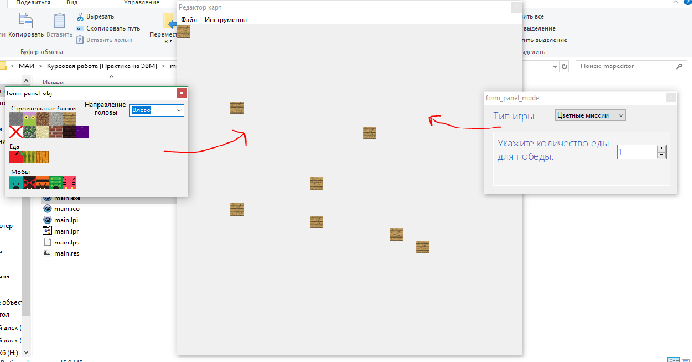
\includegraphics[scale=.9]{img1}

\caption{Скриншот редактора карт и его инструментов}
\end{center}
Здесь в форме слева можно наблюдать кнопки выбора кисти (блока, который мы сейчас будем ставить на карту). При нажатии по какой-то из кнопок, берётся значения поля Tag кнопки, затем происходит приравнивание переменной brushe из редактора к полю Tag. Когда мы открываем файл карт в редакторе карт, происходит считывание из файла служебных полей о типе игры и сразу же значения формы выбора типа игры становятся равными значениям служебных полей. Также взаимодействие происходит между главной формой и формой игрового процесса. При помощи сеттеров, главная форма задаёт выбранный сезон в игровой форме, что обеспечит загрузку карт из соответствующей папки.


\section{Основные алгоритмы}
В данной работе основными (т.е теми алгоритмами, без которых невозможно написание данной игры) являются алгоритмы, указанные ниже
\subsection{Алгоритм загрузки карты}
Цель алгоритма: обеспечить корректное открытие файла карт с проверкой данных на возможную подмену. Открытые данные расформировать по массивам.
\subsubsection{Пошаговое описание}
\textbf{Шаг 1.} Сформировать название и путь к карте по номеру сезона и номеру уровня;

\textbf{Шаг 2.} Проверить существование файла карт. Если он не найден, предупредить пользователя;

\textbf{Шаг 3.} Открыть файл, обнулить глобальные переменные количество обьектов;

\textbf{Шаг 4.} Пока не конец файла, производить чтение во временную структуру;

\textbf{Шаг 5.} Проверить поле code в структуре. Если оно равно 120, то это служебная структура, получить номер уровня, тип игры. Проверить эти данные на корректность;

\textbf{Шаг 6.} Или если получена переменная code = 18, то осуществить запись данных в переменную, отвечающую за портал;

\textbf{Шаг 7.} Или если поля code < 1 или code > 19 или vector < 1 или vector > 4, то данные являются некорректными. Уведомить пользователя в случае некорректных данных;

\textbf{Шаг 8.} Если code = 2, то данные запишутся в глобальную переменную Snake-Head при помощи конструктора;

\textbf{Шаг 9.} Иначе определить по коду тип обьекта, записать в соответсвующий массив обьектов. Мобов - в массив мобов, Блоки - в массив блоков; 

\textbf{Шаг 10.} Закрыть файл;

\textbf{Шаг 11.} Конец алгоритма;
\subsection{Алгоритм отрисовки карты}
Цель данного алгоритма - обеспечить графическое представление данных карты, находящихся в массиве. Для этого алгоритм обращается к $i$-му индексу соответствующего массива, берёт из него координаты и Bitmap.
\subsubsection{Пошаговое описание}
\textbf{Шаг 1.} Инициализировать счётчик циклов $i$;

\textbf{Шаг 2.} Для $i$ = 1 до количества блоков на форме выполнить отрисовку при помощи Canvas.Draw();

\textbf{Шаг 3.} Для $i$ = 1 до количества еды выполнить отрисовку еды на форму, при этом проверять компонент видимости. Для отрисовки он должен быть равен 1.

\textbf{Шаг 4.} Если игровой режим 2, то на свободном от блоков и змейки месте сгенерировать случайный фрукт;

\textbf{Шаг 5.} Если игровой режим 3, то проверить количество съеденных обьектов змейкой. Если оно равно необходимому, сделать компоненту видимости портала равной 1, отрисовать портал при помощи функции Canvas.Draw();

\textbf{Шаг 6.} Конец алгоритма;
\subsection{Алгоритм движения и поведения мобов}
Цель данного алгоритма - обеспечить логику поведения мобов, их принятие решений при нахождении рядом со змейкой, а также рядом со строительными блоками и фруктами
\subsubsection{Пошаговое описание}
\textbf{Шаг 1.} Для каждого моба из массива мобов выполнять следующие действия: сгенерировать случайное число в диапазоне от 1 до 100. Если будет получено число, большее чем 80, то моб должен повернуть в одно из случайных свободных для поворота направлений (т.е, направлений, которые не заняты другими мобами, блоками);

\textbf{Шаг 2.} Если встретилось некоторое препятствие (для съедобных жуков змейка также является препятствием, а для вражеских пауков нет), то посмотреть доступные направления для поворота. Среди доступных направлений случайным образом выбрать новое направление, осуществить смещение координат моба на константу BLOCK-SIZE, численно равную 24;

\textbf{Шаг 3.} Конец алгоритма;
 
\subsection{Алгоритм движения змейки}
Цель данного алгоритма - обеспечить передвижение самой змейки. Для этого используется массив обьектов хвоста и обьект головы.
\subsubsection{Пошаговое описание}
\textbf{Шаг 1.} Для $i$ = Длина змейки до 2 выполнять смещение по массиву хвоста. Иными словами, $i$-му элементу массива хвоста задаются координаты $(i-1)$-го элемента;

\textbf{Шаг 2.} Первому элементу массива задаются координаты головы;

\textbf{Шаг 3.} Координаты головы меняются в зависимости от направления движения. Иными словами, если змейка движется вверх, то меняется координата $(y:= y - 24)$, вниз: $y:= y + 24$, влево: $x:= x - 24$, вправо: $x:= x + 24$;

\textbf{Шаг 4.} Конец алгоритма
 
\subsection{Алгоритм обработки движения}
Цель данного алгоритма - контроль передвижения змейки, обработки столкновений, поеданий.
\subsubsection{Пошаговое описание}
\textbf{Шаг 1.} Проверить координаты головы на условие выхода за границы карты. Если одно из условий выполнилось, произвести смещение в другой конец карты;

\textbf{Шаг 2.} Обработать возможность столкновения змейки со своим телом. Если координаты головы совпадают с одним из элементов хвоста, игра заканчивается;

\textbf{Шаг 3.} Обработать столкновение головы с дружественными мобами. В случае столкновения, увеличить длину змейки;

\textbf{Шаг 4.} Обработать столкновения с твёрдыми блоками. При совпадении координат головы с блоком, игра заканчивается;

\textbf{Шаг 5.} Обработка столкновений с едой. При совпадении координат, увеличивается длина змейки, компонент видимости еды становится равен нулю;

\textbf{Шаг 6.} Обработка столкновений вражеских мобов со змейкой. Если координаты одного из мобов совпадают с координатами головы или хвоста змейки, игра заканчивается;

\textbf{Шаг 7.} Если игровой режим равен "Враг не дремлет", проверить совпадение координат головы змейки с координатами портала. При этом портал должен иметь компонент видимости равный 1.

\section{Руководство пользователя}
\subsection{Описание игры}
Компьютерная игра «Змейка» - мир, который управляется змеями. Здесь вам предстоит преодолеть множество препятствий, съесть немереное количество жуков и фруктов, открывать порталы, решать задачи и уничтожать все возможные преграды на пути.
\subsection{Системные требования}
Операционная система Windows 7,8,8.1,10. Для компиляции игры требуется Lazarus.
\subsection{Начало игры}
\textbf{Шаг 1.} Запустите игру
\begin{center}
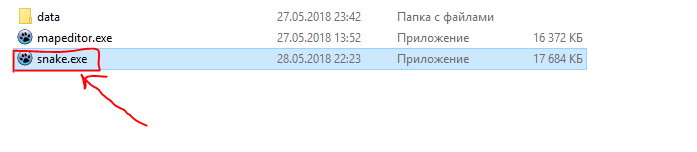
\includegraphics[scale=.9]{img2-1}
\end{center}

\textbf{Шаг 2.} Убедитесь, что у вас стоит английская раскладка клавиатуры
\begin{center}
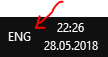
\includegraphics[scale=.9]{2-2}
\end{center}

\textbf{Шаг 3.} Вы увидите главное окно. По нему ползает главный персонаж, в центре окна располагаются кнопки начала игры, помощи и выхода. В самом низу есть кнопка отключения мелодии
\begin{center}
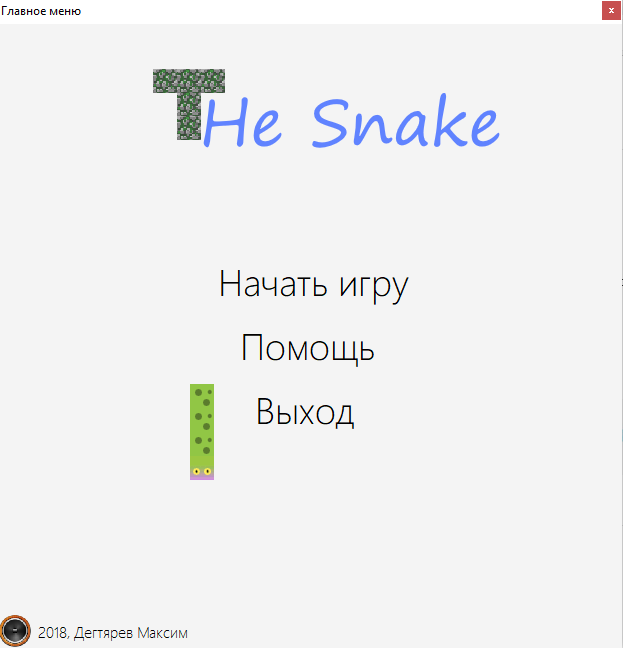
\includegraphics[scale=.9]{img2}
\end{center}

\textbf{Шаг 4.} Для начала игры кликните по кнопке "Начать игру"
\begin{center}
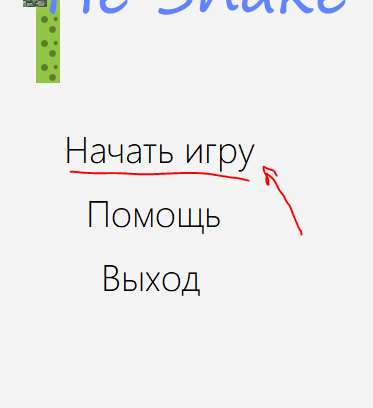
\includegraphics[scale=.9]{img5}
\end{center}

\textbf{Шаг 5.} Выберите необходимый сезон. \textit{Сезон - это набор уровней (по 5 уровней в каждом сезоне)}
\begin{center}
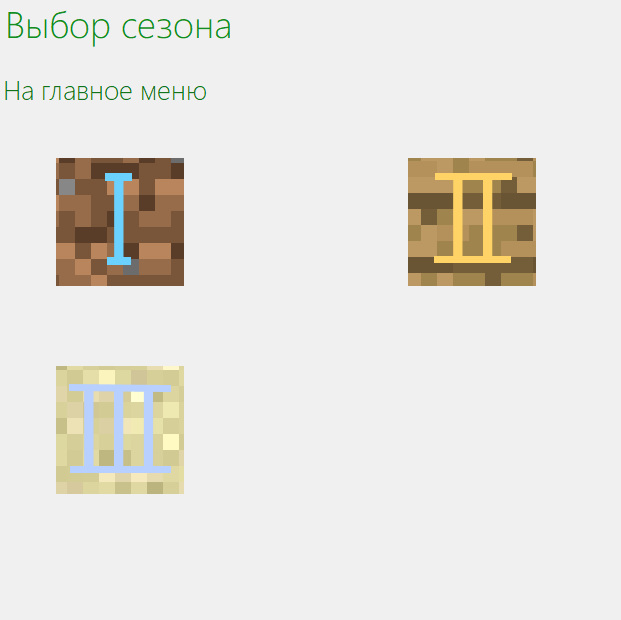
\includegraphics[scale=.9]{img3}
\end{center} 

\textbf{Шаг 6.} После выбора сезона вам будет предложено выбрать уровень для игры или вернуться к выбору сезона. Рекомендовано начинать игру с 1 уровня.
\begin{center}
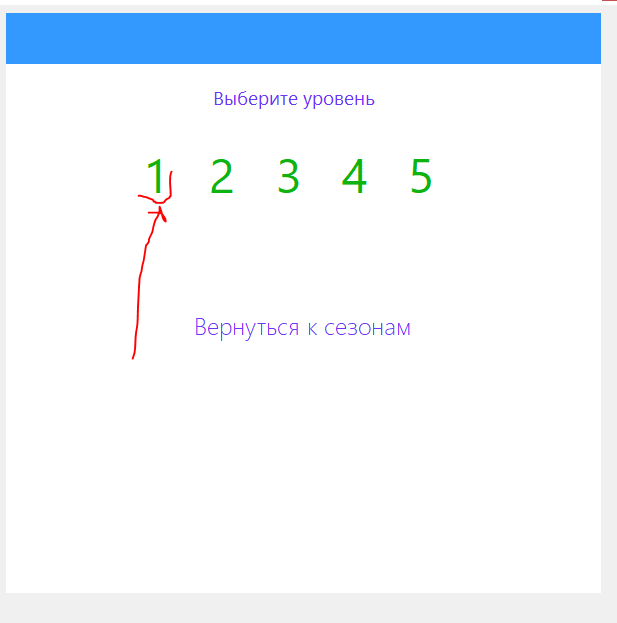
\includegraphics[scale=.9]{img6}
\end{center} 

\textbf{Шаг 7.} После выбора уровня будет открыта и загружена карта, а также для вашего удобства открыто окно с целью. Ознакомьтесь с вашей целью и нажмите кнопку начать игру (Горячая клавиша - Enter)
\begin{center}
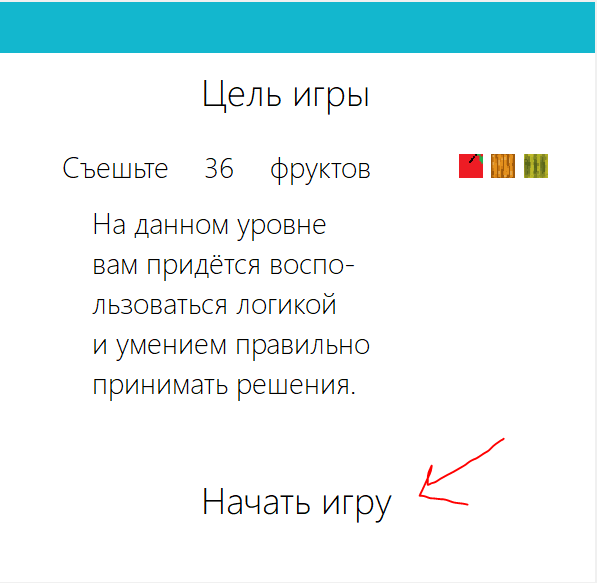
\includegraphics[scale=.9]{img7}
\end{center}

\textbf{Шаг 8.} Начнётся игра. Чтобы управлять змейкой, используйте клавиши UP, DOWN, LEFT, RIGHT. Для ускорения змейки, зажмите клавишу X. Осторожно! При быстром движении врезаться в стенку намного проще! При отпускании клавиши Z змейка будет двигаться с нормальной клавишей. На уровнях вида "Цветные миссии" клавиша Z отключена в виду её ненадобности 
\begin{center}
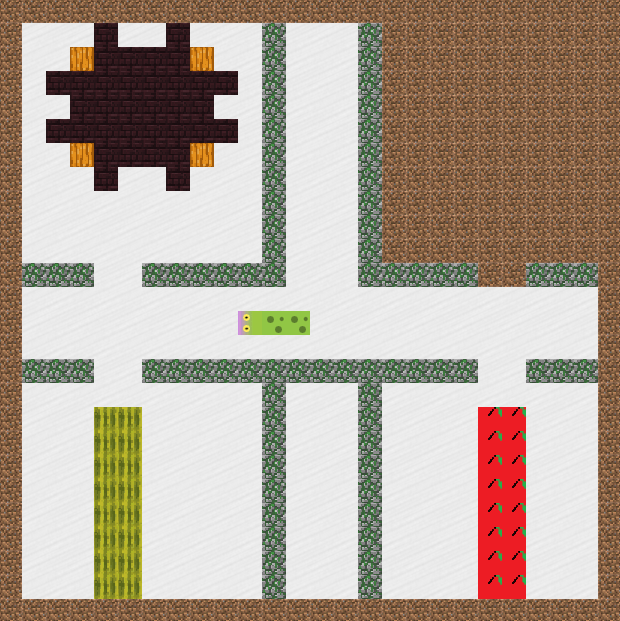
\includegraphics[scale=.9]{img8}
\end{center}

\textbf{Шаг 9.} Если у вас есть вопрос - как узнать свою цель, нажмите клавишу X. Например, так вы можете узнать, какого жука необходимо съесть на уровнях вида "Цветные миссии"
\begin{center}
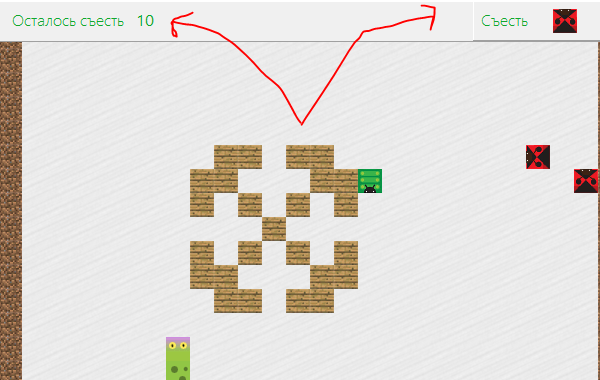
\includegraphics[scale=.9]{img9}
\end{center}

\textbf{Шаг 10.} Для того чтобы поставить игру на паузу, нажмите клавишу Esc. Будет открыто меню паузы
\begin{center}
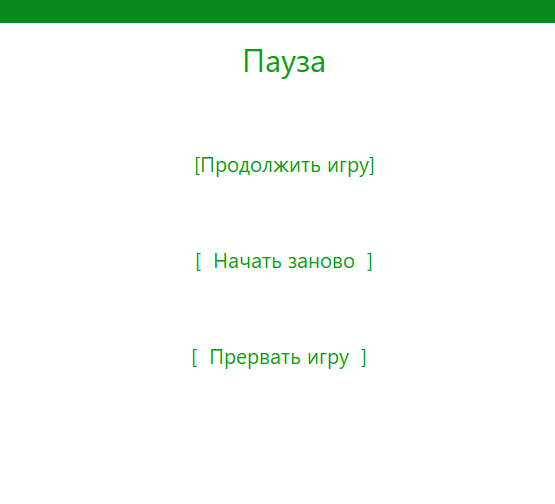
\includegraphics[scale=.9]{img10}
\end{center}

\textbf{Шаг 11.} Проходите уровень. В случае победы вам будет предложено приступить к следующему уровню или перепройти текущий
\begin{center}
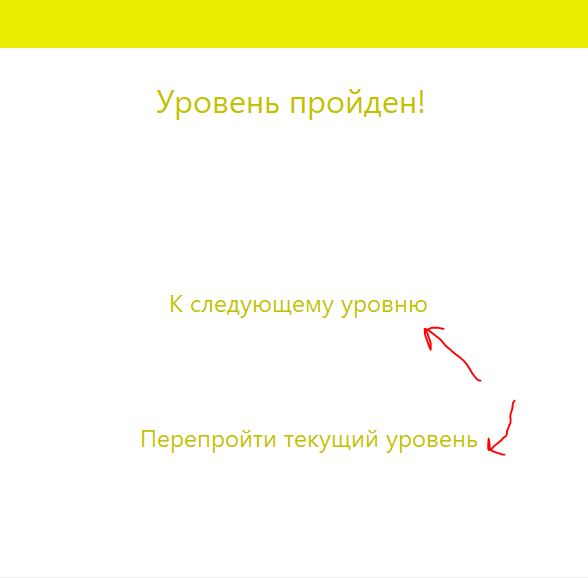
\includegraphics[scale=.9]{img11}
\end{center}

Теперь вы умеете играть в игру "The Snake". Рекомендуется пройти все уровни.
\subsection{Работа с редактором карт}
Редактор карт - утилита для разработки карт игры "The Snake".

\textbf{Шаг 1.} Откройте редактор карт
\begin{center}
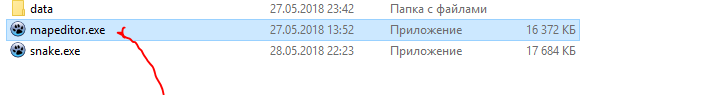
\includegraphics[scale=.9]{img12}
\end{center}

\textbf{Шаг 2.} Откроется редактор карт. Он представляет собой свободное окно с меню сверху. 
\begin{center}
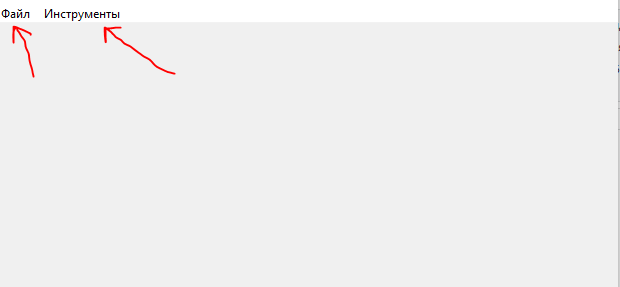
\includegraphics[scale=.9]{img13}
\end{center}

\textbf{Шаг 3.} Выберите пункт "Инструменты". Нажмите сразу по двум вкладкам
\begin{center}
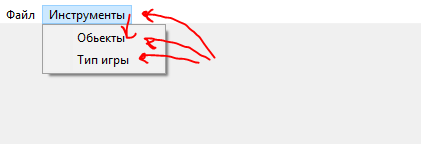
\includegraphics[scale=.9]{img14}
\end{center}

\textbf{Шаг 4.} Откроются два окна. В одном можно выбрать кисть, которой мы будем рисовать, в другом же окне - выбор типа игры, который будет происходить на карте
\begin{center}
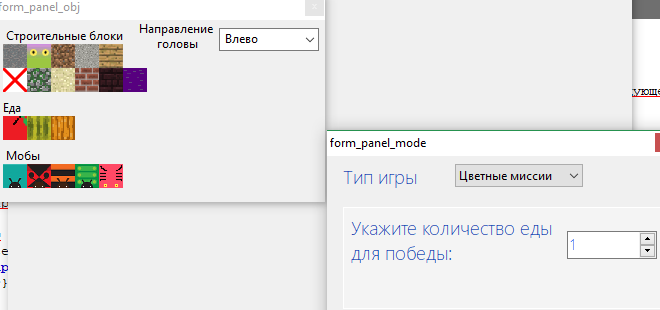
\includegraphics[scale=.9]{img15}
\end{center}

\textbf{Шаг 5.} Нарисуйте похожую карту. Учтите, что на карте обязательно нужно указать, где будет располагаться голова змейки для её корректной загрузки
\begin{center}
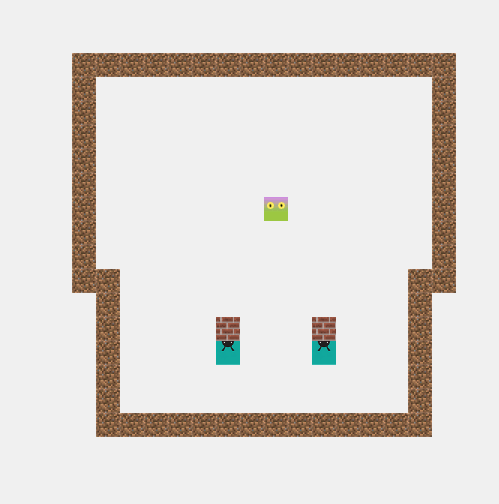
\includegraphics[scale=.9]{img16}
\end{center}

\textbf{Шаг 6.} Установите режим игры. В значении "Цель" укажите цифру 2
\begin{center}
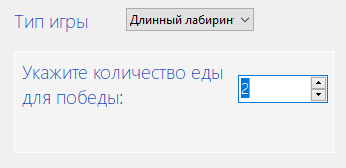
\includegraphics[scale=.9]{img17}
\end{center}

\textbf{Шаг 7.} Сохраните карту по пути: data/cards/02/. На данный момент, в змейке отдельное открытие карт недоступно. В качестве названия, напишите \verb|map_01.map|
\begin{center}
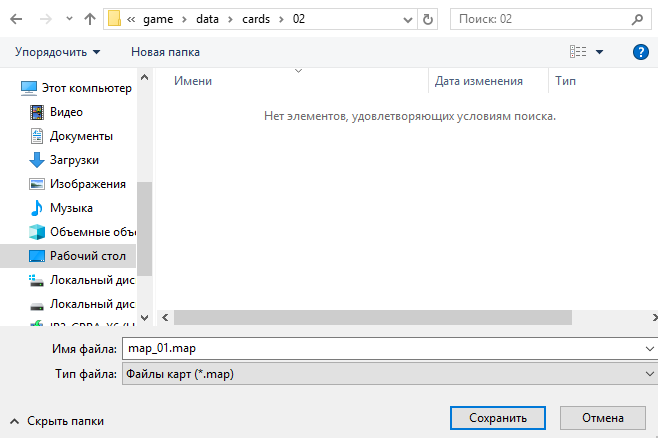
\includegraphics[scale=.9]{img18}
\end{center}

\textbf{Шаг 8.} Теперь можно поиграть в свою карту! Для этого выберите 2 сезон, уровень №1. 
\begin{center}
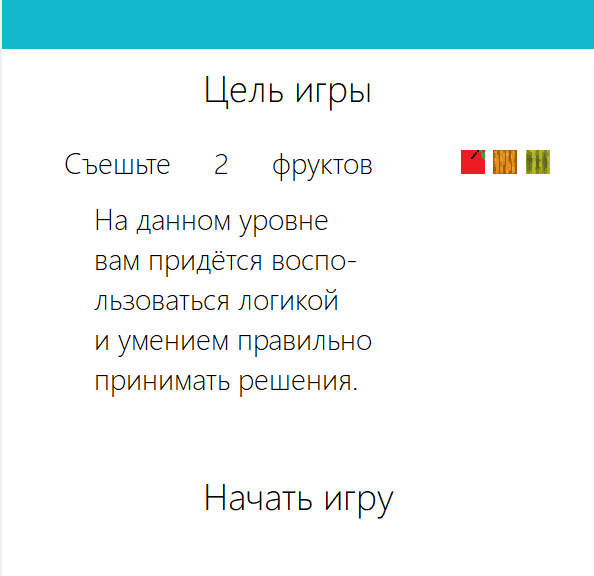
\includegraphics[scale=.9]{img19}
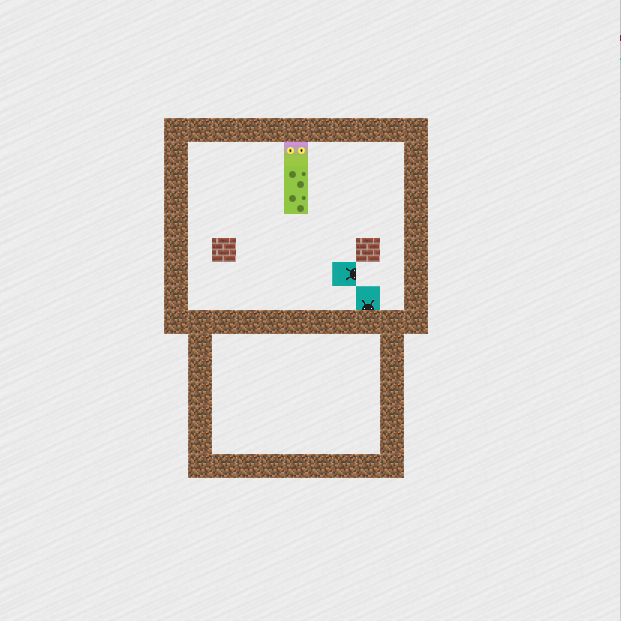
\includegraphics[scale=.9]{img20}
\end{center}
\section{Библиография} 

\subsection{Delphi}
1. Архангельский А. Я. «100 компонентов общего назначения библиотеки Delphi 5». М.: Бином, 1999, 272 стр.

2. Архангельский А. Я. «Delphi 7. Справочное пособие». М.: БиномПресс, 2003, 1024 стр.

3. Архангельский А. Я. «Приемы программирования в Delphi на основе VCL». М.: Бином-Пресс, 2009, 944 стр.

4. Архангельский А. Я. «Программирование в Delphi. Учебник по классическим версиям Delphi». М.: Бином-Пресс, 2008, 1158 стр.

5. Архангельский А. Я. «Программирование в Delphi 7». М.: БиномПресс, 2003, 1152 стр.

6. Гуриков С. Р. «Программирование в среде Lazarus для школьников и студентов. Учебное пособие». М.: Форум, 2017, 336 стр.

7. Культин Н. Б. «Delphi в задачах и примерах». СПб.: БХВ-Петербург, 2007.

8. Мансуров К. Т. «Основы программирования в среде Lazarus». М.: Palmarium Academic Publishing, 2013, 772 стр. Электронная книга

9. Фаронов В. В. «Delphi. Программирование на языке высокого уровня». СПб.: Питер, 2003, 640 стр. 

\section{Приложение}
\subsection{form-main.pas}
\begin{verbatim}
unit form_main;

{$mode objfpc}{$H+}
interface

uses
  Classes, SysUtils, FileUtil, Forms, Controls, Graphics, Dialogs, StdCtrls,
  ExtCtrls, mechanics,mmsystem;

const
  BLOCK_SIZE = 24; //Размер блока в игре
  BLOCK_COUNT = 25;
  //Количество блоков на поле. Оно есть квадрат
  SNAKE_MAX_LENGHT = 1500; //Максимальная длина змейки
  SNAKE_MIN_LENGHT = 2; //Минимальная длина змейки
  SNAKE_MAX_SPEED = 300;
  //Максимальная скорость змейки. Регулирует период таймера
  SNAKE_MIN_SPEED = 50;   //Мин.скорость

type

  { Tmain_form }
  Tmain_form = class(TForm)
    copur: TLabel;
    lb_obr: TLabel;
    lb_season: TLabel;
    lb_start1: TLabel;
    pn_seasons: TPanel;
    seas_1: TImage;
    seas_2: TImage;
    seas_3: TImage;
    shutup: TImage;
    imlogo: TImage;
    lb_start: TLabel;
    lb_start3: TLabel;
    timer_main: TTimer;
    procedure FormMouseMove(Sender: TObject; Shift: TShiftState; X, Y: integer);
    procedure FormPaint(Sender: TObject);
    procedure lb_obrClick(Sender: TObject);
    procedure lb_startMouseLeave(Sender: TObject);
    procedure seas_1Click(Sender: TObject);
    procedure shutupClick(Sender: TObject);
    procedure StartGame;
    procedure Move;
    procedure OnMove;

    procedure btn_startgmClick(Sender: TObject);
    procedure btn_editClick(Sender: TObject);
    procedure FormCreate(Sender: TObject);
    procedure lb_startClick(Sender: TObject);
    procedure lb_startMouseEnter(Sender: TObject);
    procedure timer_mainTimer(Sender: TObject);
  private

  public

  end;

var
  main_form: Tmain_form;
  Snake_Tail: array[1..10] of TTail; //Массив есть хвост
  Snake_Head: THead;
  PApple, PMelon, PPumpkin, PHead, PTail: TBitmap;
  Lenght: integer;
  vect: integer;
  cx, cy: integer;
  music: boolean;
implementation

uses
  form_game_mode_2, help;

{$R *.lfm}

{ Tmain_form }

procedure startGameMusic;
begin
  sndPlaySound('data/sounds/main.wav', SND_ASYNC or SND_NODEFAULT);
end;
procedure stopGameMusic;
begin
  sndPlaySound(nil,0);
end;

procedure Tmain_form.OnMove;
var
  i: integer;
begin
  {Обработка выхода за границы карты}
  if (Snake_Head.getX = Width) then
  begin
    Snake_Head.setX(abs(Snake_Head.getX - Width));
  end
  else if (Snake_Head.getX < 0) then
  begin
    Snake_Head.setX(Width);
  end
  else if (Snake_Head.getY = Height) then
  begin
    Snake_Head.setY(abs(Snake_Head.getY - Height));
  end
  else if (Snake_Head.getY < 0) then
  begin
    Snake_Head.SetY(Height);
  end;

  for i:= 2 to Lenght do begin;
  if ((Snake_Head.getX = CX) and (Snake_Head.getY = CY)) or ((Snake_Tail[i].getX = CX) and (Snake_Tail[i].getY = CY)) then begin
    timer_main.Interval:=20;
  end
  else
  timer_main.Interval:=300;
  end;
end;

procedure Tmain_form.Move;
var
  i: integer;
begin
  {Переписывание кординат для будущей отрисовки}
  for i := Lenght downto SNAKE_MIN_LENGHT do
  begin
    Snake_Tail[i].setX(Snake_Tail[i - 1].getX);
    Snake_Tail[i].setY(Snake_Tail[i - 1].getY);
  end;

  {Обновление окологоловного элемента}
  with Snake_Tail[1] do
  begin
    setX(Snake_Head.getX);
    setY(Snake_Head.getY);
  end;

  {Контроль прибавления пикселей}
  case Vect of
    1: Snake_Head.setX(Snake_Head.getX - BLOCK_SIZE);
    2: Snake_Head.setX(Snake_Head.getX + BLOCK_SIZE);
    3: Snake_Head.setY(Snake_Head.getY - BLOCK_SIZE);
    4: Snake_Head.setY(Snake_Head.getY + BLOCK_SIZE);
  end;
end;

procedure Tmain_form.StartGame;
var
  coord_x, coord_y: integer;
begin
  Lenght := 3;
  PHeadUp := TBitmap.Create();
  PHeadDown := TBitmap.Create();
  PHeadLeft := TBitmap.Create();
  PHeadRigth := TBitmap.Create();
  PTail := TBitmap.Create();
  PApple := TBitmap.Create();
  PMelon := TBitmap.Create();
  PPumpkin := TBitmap.Create();
  PHeadUp.LoadFromFile('data/sprites/head_up.bmp');
  PHeadDown.LoadFromFile('data/sprites/head_down.bmp');
  PHeadLeft.LoadFromFile('data/sprites/head_left.bmp');
  PHeadRigth.LoadFromFile('data/sprites/head_rigth.bmp');
  PTail.LoadFromFile('data/sprites/body.bmp');
  PApple.LoadFromFile('data/sprites/apple.bmp');
  PMelon.LoadFromFile('data/sprites/watermelon.bmp');
  PPumpkin.LoadFromFile('data/sprites/pumpkin.bmp');
  randomize;
  vect := 1 + Random(4);

  //Случайные координаты головы
  coord_x := Random(BLOCK_COUNT + 1) * BLOCK_SIZE;
  coord_y := Random(BLOCK_COUNT + 1) * BLOCK_SIZE;

  case vect of
    1:
      Snake_Head := THead.Init(coord_x, coord_y, 1, PHeadLeft);
    2:
      Snake_Head := THead.Init(coord_x, coord_y, 1, PHeadRigth);
    3:
      Snake_Head := THead.Init(coord_x, coord_y, 1, PHeadUp);
    4:
      Snake_Head := THead.Init(coord_x, coord_y, 1, PHeadDown);
  end;

  case vect of
    1:
    begin
      Snake_Tail[1] := TTail.Init(Snake_Head.getX + BLOCK_SIZE,
        Snake_Head.getY, 1, PTail);
      Snake_Tail[2] := TTail.Init(Snake_Head.getX + 2 * BLOCK_SIZE,
        Snake_Head.getY, 1, PTail);
      Snake_Tail[3] := TTail.Init(Snake_Head.getX + 3 * BLOCK_SIZE,
        Snake_Head.getY, 1, PTail);
    end;
    2:
    begin
      Snake_Tail[1] := TTail.Init(Snake_Head.getX - BLOCK_SIZE,
        Snake_Head.getY, 1, PTail);
      Snake_Tail[2] := TTail.Init(Snake_Head.getX - 2 * BLOCK_SIZE,
        Snake_Head.getY, 1, PTail);
      Snake_Tail[3] := TTail.Init(Snake_Head.getX - 3 * BLOCK_SIZE,
        Snake_Head.getY, 1, PTail);
    end;
    3:
    begin
      Snake_Tail[1] := TTail.Init(Snake_Head.getX, Snake_Head.getY +
        BLOCK_SIZE, 1, PTail);
      Snake_Tail[2] := TTail.Init(Snake_Head.getX, Snake_Head.getY +
        2 * BLOCK_SIZE, 1, PTail);
      Snake_Tail[3] := TTail.Init(Snake_Head.getX, Snake_Head.getY +
        3 * BLOCK_SIZE, 1, PTail);
    end;
    4:
    begin
      Snake_Tail[1] := TTail.Init(Snake_Head.getX, Snake_Head.getY -
        BLOCK_SIZE, 1, PTail);
      Snake_Tail[2] := TTail.Init(Snake_Head.getX, Snake_Head.getY -
        2 * BLOCK_SIZE, 1, PTail);
      Snake_Tail[3] := TTail.Init(Snake_Head.getX, Snake_Head.getY -
        3 * BLOCK_SIZE, 1, PTail);
    end;
  end;

end;

procedure Tmain_form.FormPaint(Sender: TObject);
var
  i: integer;
begin
  {Отрисовываем хвост}
  for i := 1 to Lenght do
    Canvas.Draw(Snake_Tail[i].getX, Snake_Tail[i].getY, Snake_Tail[i].getBitmap);

  {Отрисовка головы}
  Canvas.Draw(Snake_Head.getX, Snake_Head.getY, Snake_Head.getBitmap);
end;

procedure Tmain_form.lb_obrClick(Sender: TObject);
begin
  pn_seasons.Visible:=False;
end;

procedure Tmain_form.FormMouseMove(Sender: TObject; Shift: TShiftState; X, Y: integer);

begin
  cx := X - (X mod BLOCK_SIZE);
  cy := Y - (Y mod BLOCK_SIZE);
end;

procedure Tmain_form.lb_startMouseLeave(Sender: TObject);
begin
  (Sender as TLabel).Font.Color := RGBToColor(0, 0, 0);
end;

procedure Tmain_form.seas_1Click(Sender: TObject);
begin
  game_mode_2_form.SetGameSeason((Sender as TImage).Tag);
  game_mode_2_form.Show;
  Self.Visible:=false;
end;

procedure Tmain_form.shutupClick(Sender: TObject);
begin
  if music = true then
     begin
       stopGameMusic;
       music:=false;
     end
  else
  begin
       startGameMusic;
       music:=True;
  end;
end;

procedure Tmain_form.btn_editClick(Sender: TObject);
begin
  //redact.Show;
end;

procedure Tmain_form.FormCreate(Sender: TObject);
begin
  {Основные задачи}
  DoubleBuffered := True; //Буферизация
  startGameMusic;
  music:=true;
  Width := BLOCK_SIZE * (BLOCK_COUNT + 1);
  Height := Width;
  StartGame;
end;


procedure Tmain_form.lb_startClick(Sender: TObject);
begin
  stopGameMusic;
  case (Sender as TLabel).Tag of
    1: pn_seasons.Visible:=true;
    2: helpform.Show;
    4: Self.Close;
  end;

end;

procedure Tmain_form.lb_startMouseEnter(Sender: TObject);
begin
  (Sender as TLabel).Font.Color := TColor($0015B72E);
end;

procedure Tmain_form.timer_mainTimer(Sender: TObject);
var
  i: integer;
  tempv: integer;
begin
  Inc(i);
  if i >= 4 + Random(8) then
  begin
    tempv := 1 + Random(4);
    i := 0;
    case tempv of
      4:
      begin
        if (Vect <> 3) then
        begin
          Vect := 4;
          Snake_Head.setBitmap(PHeadDown);
        end;
      end;
      2:
      begin
        if (Vect <> 1) then
        begin
          Vect := 2;
          Snake_Head.setBitmap(PHeadRigth);
        end;
      end;
      3:
      begin
        if (Vect <> 4) then
        begin
          Vect := 3;
          Snake_Head.setBitmap(PHeadUp);
        end;
      end;
      1:
      begin
        if (Vect <> 2) then
        begin
          Vect := 1;
          Snake_Head.setBitmap(PHeadLeft);
        end;
      end;
    end;
  end;

  Move;
  OnMove;
  Refresh;

end;
end.
\end{verbatim}
\subsection{mechanics.pas}
\begin{verbatim}
unit mechanics;

{
     2018, Максим Дегтярев
     Основные классы игры
}
{$mode objfpc}{$H+}

interface

uses
  Classes, SysUtils, Graphics;

type

  { TBase }
  TAbstract = class
    private
      x : Integer;
      y : Integer;
      bitmap : TBitmap;
      viscomp: integer;
      mode: Integer;
    public

      {Constructor}
      Constructor Init(x0,y0, v0 : Integer; texture : TBitmap);

      {Setters}
      procedure setX(x0 : Integer);
      procedure setY(y0 : Integer);
      procedure setVisComp(v0: Integer);
      procedure setBitmap(texture : TBitmap);
      procedure SetMode(value: integer);
      {Getters}
      function getX : Integer;
      function getY : Integer;
      function getVisComp: Integer;
      function getMode: Integer;
      function getBitmap : TBitmap;
  end;

  TFood = class (TAbstract) end;

  TBlock = class (TAbstract) end;

  TMob = class (TAbstract)
  private
    myvect, codemob: integer; //Направление движения моба, код моба
  public
    procedure setVect(me: integer);
    procedure setCodeMob(me: integer);

    function getCodeMob: integer;
    function getVect: integer;
  end;

  THead = class (TAbstract) end;

  TTail = class (TAbstract) end;
implementation

{ TAbstract }

{Functions}
constructor TAbstract.Init(x0, y0, v0: Integer; texture: TBitmap);
begin
  x := x0;
  y := y0;
  viscomp:=v0;
  bitmap := texture;
end;

procedure TAbstract.setX(x0: Integer);
begin
  x := x0;
end;

procedure TAbstract.setY(y0: Integer);
begin
  y := y0;
end;

procedure TAbstract.setVisComp(v0: integer);
begin
  viscomp:=v0;
end;

procedure TAbstract.SetMode(value: integer);
begin
  mode:=value;
end;

procedure TAbstract.setBitmap(texture: TBitmap);
begin
  bitmap := texture;
end;

function TAbstract.getX: Integer;
begin
  Result := x;
end;

function TAbstract.getY: Integer;
begin
  Result := y;
end;

function TAbstract.getMode: Integer;
begin
  result:= mode;
end;

function TAbstract.getVisComp: Integer;
begin
  Result:= viscomp;
end;

function TAbstract.getBitmap: TBitmap;
begin
  Result := bitmap;
end;

//Для моба

procedure TMob.setCodeMob(me: integer);
begin
  codemob:=me;
end;

procedure TMob.setVect(me: integer);
begin
  myvect:=me;
end;

function TMob.getCodeMob: integer;
begin
  result:= codemob;
end;

function TMob.getVect: integer;
begin
  result:= myvect;
end;
end.
\end{verbatim}
\subsection{form-game-mode-2.pas}
\begin{verbatim}
unit form_game_mode_2;

{$mode objfpc}{$H+}

interface

uses
  Classes, SysUtils, FileUtil, Forms, Controls, Graphics, Dialogs, ExtCtrls,
  StdCtrls, mechanics, mmsystem;

{Основные игровые константы}
const
  BLOCK_SIZE = 24; //Размер блока в игре
  BLOCK_COUNT = 25;
  //Количество блоков на поле. Оно есть квадрат
  SNAKE_MAX_LENGHT = 1500; //Максимальная длина змейки
  SNAKE_MIN_LENGHT = 2; //Минимальная длина змейки
  SNAKE_MAX_SPEED = 300;
  //Максимальная скорость змейки. Регулирует период таймера
  SNAKE_MIN_SPEED = 50;   //Мин.скорость

type
  mapobj = record
    x, y: integer; //Координаты
    code: integer; //Тип обьекта
    vector: integer;
    //Куда будет направлена голова змейки (если это голова)
    cel: integer; //-368
    plan: integer;
    mapcode: integer;
  end;
  { Tgame_mode_2_form }

  Tgame_mode_2_form = class(TForm)
    cell: TImage;
    gameoverp: TPanel;
    gamepause: TPanel;
    gamewin: TPanel;
    gmpn: TPanel;
    lb_o4ki1: TLabel;
    lb_ost: TLabel;
    lb_ost_n: TLabel;
    N1: TLabel;
    N3: TLabel;
    N4: TLabel;
    N: TLabel;
    _lv1: TLabel;
    _lv2: TLabel;
    _lv5: TLabel;
    _lv6: TLabel;
    _lv7: TLabel;
    _lv_exit1: TLabel;
    _startgame2: TLabel;
    _startgame4: TLabel;
    _startgame5: TLabel;
    _title: TLabel;
    _title12: TLabel;
    _title13: TLabel;
    _title14: TLabel;
    _title15: TLabel;
    _title16: TLabel;
    _title17: TLabel;
    _title18: TLabel;
    _title19: TLabel;
    procedure FormClose(Sender: TObject; var CloseAction: TCloseAction);
    procedure FormCreate(Sender: TObject);
    procedure FormKeyDown(Sender: TObject; var Key: word; Shift: TShiftState);
    procedure FormKeyPress(Sender: TObject; var Key: char);
    procedure FormKeyUp(Sender: TObject; var Key: word; Shift: TShiftState);
    procedure FormMouseDown(Sender: TObject; Button: TMouseButton;
      Shift: TShiftState; X, Y: integer);
    procedure FormPaint(Sender: TObject);
    procedure lb_restartClick(Sender: TObject);
    procedure timer_keyboardTimer(Sender: TObject);
    procedure timer_mainTimer(Sender: TObject);
    procedure timer_realTimer(Sender: TObject);
    procedure _lv1Click(Sender: TObject);
    procedure OpenCard(crd: string);
    procedure LoadMap;
    procedure StartGame;
    procedure GameOver;
    procedure Move;
    procedure MobsMove;
    procedure AddTail;
    procedure OnMove;
    procedure SuccessFull;
    procedure NextLevel;
    procedure KillerMove;
    procedure KillerSetVector(id: integer);

    procedure _lv_exitClick(Sender: TObject);
    procedure _startgame1Click(Sender: TObject);
    procedure _startgame2Click(Sender: TObject);
    procedure _startgame3Click(Sender: TObject);
    procedure _startgame5Click(Sender: TObject);
    procedure _title2Click(Sender: TObject);
    procedure _title3Click(Sender: TObject);
    procedure _title4Click(Sender: TObject);
    procedure _title5Click(Sender: TObject);
    procedure _title7Click(Sender: TObject);
    procedure _title8Click(Sender: TObject);
    procedure mobSetVect(id: integer);

    procedure PlaceFood;
    procedure PlaceMobs(which: integer);
    procedure SetGameSeason(season: integer);
    procedure ClearGame;
    procedure GenCell;

  private

  public

  end;

var
  game_mode_2_form: Tgame_mode_2_form;

  BLOCKS_ON_FORM: integer;
  Objects: array of mapobj; //Массив обьектов
  BL_ON_FORM: integer;
  FOOD_ON_FORM: integer;
  MOBS_ON_FORM: integer;
  KILLERS_ON_FORM: integer;

  Lenght: integer; //Хранит длину змейки

  UsedHead: boolean;
  //Маячок - открыт ли ресурс "голова" и считаны ли координаты?

  {Что нужно съесть из жуков змейке}
  Snake_Cell: integer; //Просто номер
  {Спрайты}
  Snake_Tail: array[1..SNAKE_MAX_LENGHT] of TTail; //Массив есть хвост
  Snake_Food: array[1..SNAKE_MAX_LENGHT] of TFood;  //Массив еды
  Snake_Blocks: array[1..SNAKE_MAX_LENGHT] of TBlock; //Массив блоков
  Snake_Mobs: array[1..SNAKE_MAX_LENGHT] of TMob; //Массив мобов
  Snake_Killers: array[1..SNAKE_MAX_LENGHT] of TMob;
  //Массив вражеских мобов
  Snake_Head: THead;
  SpFood: TFood;
  SpPortal: TBlock; //Блок портала
  Coords: array[1..SNAKE_MAX_LENGHT] of mapobj;
  Coords_k: array[1..SNAKE_MAX_LENGHT] of mapobj;

  {Текстуры}
  PMobKiller1_left, PMobKiller1_right, PMobKiller1_up, PMobKiller1_down,
  PMob4_left, PMob4_right, PMob4_up, PMob4_down, PMob3_left, PMob3_right,
  PMob3_up, PMob3_down, PMob2_left, PMob2_right, PMob2_up, PMob2_down,
  PMob_left, PMob_right, PMob_up, PMob_down, PBackground, PPortalBefore,
  PPortalAfter, PApple, PMelon, PPumpkin, PStone, PHeadUp, PTail,
  PFood, PHeadDown, PHeadLeft, PHeadRigth, PTerrain, PWall, PTree,
  PNowHead, PGreenStone, PSand, PBrick, PRedBrick: TBitmap;

  //Вектор
  vect: integer;

  //Начата ли игра?
  StartedGame: boolean;
  PausedGame: boolean;



  {Что получаем при выгрузке головы из файла}
  GV, onstart_x, onstart_y: integer;

  {Служебные переменные}
  GameMode: integer; //Режим игры
  GamePlan: integer; //Цель игры

  {Служебные переменные об номере уровня, сезона}
  GameLevel: integer; //Текущий уровень
  GameSeason: integer; //Текущий сезон

  {Решение проблемы с клавиатурой - залипание}
  GameKeyZalip: boolean; //Залипание клавиши

implementation

uses
  form_main;

{$R *.lfm}
{Отдельный блок для звуков}
procedure winSound;
begin
  sndPlaySound('data/sounds/level_complete.wav', SND_ASYNC or SND_NODEFAULT);
end;

procedure failSound;
begin
  sndPlaySound('data/sounds/level_failed.wav', SND_ASYNC or SND_NODEFAULT);
end;

procedure stopGameMusic;
begin
  sndPlaySound(nil, 0);
end;

{ Tgame_mode_2_form }

{Записать обьекты в массив обьектов. Времени мало, не самое эффективное}
procedure InsertObjects;
var
  i: integer;
begin
  Objects := nil;
  BLOCKS_ON_FORM := 0;

  for i := 1 to BL_ON_FORM do
  begin
    Inc(BLOCKS_ON_FORM);
    SetLength(Objects, BLOCKS_ON_FORM);
    with Objects[BLOCKS_ON_FORM - 1] do
    begin
      x := Snake_Blocks[i].getX;
      y := Snake_Blocks[i].getY;
    end;
  end;

  for i := 1 to FOOD_ON_FORM do
  begin
    if Snake_Food[i].getVisComp = 1 then begin
    Inc(BLOCKS_ON_FORM);
    SetLength(Objects, BLOCKS_ON_FORM);
    with Objects[BLOCKS_ON_FORM - 1] do
    begin
      x := Snake_Food[i].getX;
      y := Snake_Food[i].getY;
    end;
    end;
  end;

  for i := 1 to MOBS_ON_FORM do
  begin
    if Snake_Mobs[i].getVisComp = 1 then begin
    Inc(BLOCKS_ON_FORM);
    SetLength(Objects, BLOCKS_ON_FORM);
    with Objects[BLOCKS_ON_FORM - 1] do
    begin
      x := Snake_Mobs[i].getX;
      y := Snake_Mobs[i].getY;
    end;
    end;
  end;

  //Вражеские мобы
  for i := 1 to KILLERS_ON_FORM do
  begin
    Inc(BLOCKS_ON_FORM);
    SetLength(Objects, BLOCKS_ON_FORM);
    with Objects[BLOCKS_ON_FORM - 1] do
    begin
      x := Snake_Killers[i].getX;
      y := Snake_Killers[i].getY;
    end;
  end;
  //Теперь сам хвост
  for i := 1 to Lenght - 1 do
  begin
    Inc(BLOCKS_ON_FORM);
    SetLength(Objects, BLOCKS_ON_FORM);
    with Objects[BLOCKS_ON_FORM - 1] do
    begin
      x := Snake_Tail[i].getX;
      y := Snake_Tail[i].getY;
    end;
  end;

  Inc(BLOCKS_ON_FORM);
  SetLength(Objects, BLOCKS_ON_FORM);
  with Objects[BLOCKS_ON_FORM - 1] do
  begin
    x := Snake_Head.getX;
    y := Snake_Head.getY;
  end;
end;

//Проверяет, свободны ли от блока координаты?
function IsFreeCoords(A, B: integer): boolean;
var
  i: integer;
begin
  InsertObjects;
  Result := True;

  for i := 0 to BLOCKS_ON_FORM - 1 do
  begin
    if (Objects[i].x = A) and (Objects[i].y = B) then
    begin
      Result := False;
      break;
    end;
  end;
end;

//Проверяет, свободные ли от блока координаты (без учёта змейки)
function IsFreeCoordsNoSnake(A, B: integer): boolean;
var
  i: integer;
begin
  Objects := nil;
  BLOCKS_ON_FORM := 0;

  for i := 1 to BL_ON_FORM do
  begin
    Inc(BLOCKS_ON_FORM);
    SetLength(Objects, BLOCKS_ON_FORM);
    with Objects[BLOCKS_ON_FORM - 1] do
    begin
      x := Snake_Blocks[i].getX;
      y := Snake_Blocks[i].getY;
    end;
  end;

  for i := 1 to FOOD_ON_FORM do
  begin
    if Snake_Food[i].getVisComp = 1 then begin
    Inc(BLOCKS_ON_FORM);
    SetLength(Objects, BLOCKS_ON_FORM);
    with Objects[BLOCKS_ON_FORM - 1] do
    begin
      x := Snake_Food[i].getX;
      y := Snake_Food[i].getY;
    end;
    end;
  end;

  for i := 1 to MOBS_ON_FORM do
  begin
    if Snake_Mobs[i].getVisComp = 1 then begin
    Inc(BLOCKS_ON_FORM);
    SetLength(Objects, BLOCKS_ON_FORM);
    with Objects[BLOCKS_ON_FORM - 1] do
    begin
      x := Snake_Mobs[i].getX;
      y := Snake_Mobs[i].getY;
    end;
    end;
  end;

  //Вражеские мобы
  for i := 1 to KILLERS_ON_FORM do
  begin
    Inc(BLOCKS_ON_FORM);
    SetLength(Objects, BLOCKS_ON_FORM);
    with Objects[BLOCKS_ON_FORM - 1] do
    begin
      x := Snake_Killers[i].getX;
      y := Snake_Killers[i].getY;
    end;
  end;
  Result := True;

  for i := 0 to BLOCKS_ON_FORM - 1 do
  begin
    if (Objects[i].x = A) and (Objects[i].y = B) then
    begin
      Result := False;
      break;
    end;
  end;
end;

function IsFreeCoordsKeyB(A, B: integer): boolean;
var
  i: integer;
begin
  Objects := nil;
  BLOCKS_ON_FORM := 0;

  for i := 1 to BL_ON_FORM do
  begin
    Inc(BLOCKS_ON_FORM);
    SetLength(Objects, BLOCKS_ON_FORM);
    with Objects[BLOCKS_ON_FORM - 1] do
    begin
      x := Snake_Blocks[i].getX;
      y := Snake_Blocks[i].getY;
    end;
  end;

  Result := True;

  for i := 0 to BLOCKS_ON_FORM - 1 do
  begin
    if (Objects[i].x = A) and (Objects[i].y = B) then
    begin
      Result := False;
      break;
    end;
  end;
end;
procedure Tgame_mode_2_form.KillerSetVector(id: integer);
var
  chose: set of 10..11;
  temp,i,k: integer;
begin
  Randomize;
  k:= 4;
  temp:= Snake_Killers[id].getVect;

  if (IsFreeCoordsNoSnake(Snake_Killers[id].getX - BLOCK_SIZE,
    Snake_Killers[id].getY)) and (Snake_Killers[id].getVect <> 1) and
    (Snake_Killers[id].getX <> 0) then
  begin
    chose:= chose + [1];
  end;
  if (IsFreeCoordsNoSnake(Snake_Killers[id].getX + BLOCK_SIZE,
    Snake_Killers[id].getY)) and (Snake_Killers[id].getVect <> 2) and
    (Snake_Killers[id].getX <> Width) then
  begin
    chose:= chose + [2];
  end;
  if (IsFreeCoordsNoSnake(Snake_Killers[id].getX, Snake_Killers[id].getY -
    BLOCK_SIZE)) and (Snake_Killers[id].getVect <> 3) and
    (Snake_Killers[id].getY <> 0) then
  begin
    chose:= chose + [3];
  end;
  if (IsFreeCoordsNoSnake(Snake_Killers[id].getX, Snake_Killers[id].getY +
    BLOCK_SIZE)) and (Snake_Killers[id].getVect <> 4) and
    (Snake_Killers[id].getY <> Height) then
  begin
    chose:= chose + [4];
  end;


  for i:= 1 to 50 do begin
    temp:= 1 + Random(k);
    if temp in chose then begin
        Snake_Killers[id].setVect(temp);
        break;
    end
    else
    Snake_Killers[id].setVect(0);
  end;

  case Snake_Killers[id].getVect of
    1:
      Snake_Killers[id].setX(Snake_Killers[id].getX - BLOCK_SIZE);
    2:
      Snake_Killers[id].setX(Snake_Killers[id].getX + BLOCK_SIZE);
    3:
      Snake_Killers[id].setY(Snake_Killers[id].getY - BLOCK_SIZE);
    4:
      Snake_Killers[id].setY(Snake_Killers[id].getY + BLOCK_SIZE);
  end;

  //Устанавливаем новый битмап
  setBitmapByMob(Snake_Killers[id], Snake_Killers[id].getVect);
end;

//Устанавливает новый вектор, производит смещение
procedure Tgame_mode_2_form.mobSetVect(id: integer);
var
  chose: set of 10..11;
  temp,i,k: integer;
begin

  k:= 4;
  temp:= Snake_Mobs[id].getVect;

  if (IsFreeCoords(Snake_Mobs[id].getX - BLOCK_SIZE, Snake_Mobs[id].getY)) and
    (Snake_Mobs[id].getVect <> 1) and (Snake_Mobs[id].getX <> 0) then
  begin
    chose:= chose + [1];
  end;
  if (IsFreeCoords(Snake_Mobs[id].getX + BLOCK_SIZE, Snake_Mobs[id].getY)) and
    (Snake_Mobs[id].getVect <> 2) and (Snake_Mobs[id].getX <> Width) then
  begin
    chose:= chose + [2];
  end;
  if (IsFreeCoords(Snake_Mobs[id].getX, Snake_Mobs[id].getY - BLOCK_SIZE)) and
    (Snake_Mobs[id].getVect <> 3) and (Snake_Mobs[id].getY <> 0) then
  begin
    chose:= chose + [3];
  end;
  if (IsFreeCoords(Snake_Mobs[id].getX, Snake_Mobs[id].getY + BLOCK_SIZE)) and
    (Snake_Mobs[id].getVect <> 4) and (Snake_Mobs[id].getY <> Height) then
  begin
    chose:= chose + [4];
  end;

    for i:= 1 to 50 do begin
    temp:= 1 + Random(k);
    if temp in chose then begin
        Snake_Mobs[id].setVect(temp);
        break;
    end
    else
    Snake_Mobs[id].setVect(0);
  end;

  case Snake_Mobs[id].getVect of
    1:
      Snake_Mobs[id].setX(Snake_Mobs[id].getX - BLOCK_SIZE);
    2:
      Snake_Mobs[id].setX(Snake_Mobs[id].getX + BLOCK_SIZE);
    3:
      Snake_Mobs[id].setY(Snake_Mobs[id].getY - BLOCK_SIZE);
    4:
      Snake_Mobs[id].setY(Snake_Mobs[id].getY + BLOCK_SIZE);
  end;

  //Устанавливаем новый битмап
  setBitmapByMob(Snake_Mobs[id], Snake_Mobs[id].getVect);
end;


procedure Tgame_mode_2_form.MobsMove;
var
  i: integer;
begin
  //Обрабатываем движение каждого моба
  Randomize;
  for i := 1 to MOBS_ON_FORM do
  begin
    if Random(100) > 80 then
    begin
      Snake_Mobs[i].setVect(1 + Random(4));
      setBitmapByMob(Snake_Mobs[i], Snake_Mobs[i].getVect);
    end;
    case Snake_Mobs[i].getVect of
      1:
      begin //Если координаты свободны влево, то тогда двигаем влево
        if IsFreeCoords(Snake_Mobs[i].getX - BLOCK_SIZE, Snake_Mobs[i].getY) and
          (Snake_Mobs[i].getX <> 0) then
        begin
          Snake_Mobs[i].setX(Snake_Mobs[i].getX - BLOCK_SIZE);
        end
        else
          mobSetVect(i);
      end;
      2:
      begin
        if IsFreeCoords(Snake_Mobs[i].getX + BLOCK_SIZE, Snake_Mobs[i].getY) and
          (Snake_Mobs[i].getX <> Width) then
        begin
          Snake_Mobs[i].setX(Snake_Mobs[i].getX + BLOCK_SIZE);
        end
        else
          mobSetVect(i);
      end;
      3:
      begin
        if IsFreeCoords(Snake_Mobs[i].getX, Snake_Mobs[i].getY - BLOCK_SIZE) and
          (Snake_Mobs[i].getY <> 0) then
        begin
          Snake_Mobs[i].setY(Snake_Mobs[i].getY - BLOCK_SIZE);
        end
        else
          mobSetVect(i);
      end;
      4:
      begin
        if IsFreeCoords(Snake_Mobs[i].getX, Snake_Mobs[i].getY + BLOCK_SIZE) and
          (Snake_Mobs[i].getY <> Height) then
        begin
          Snake_Mobs[i].setY(Snake_Mobs[i].getY + BLOCK_SIZE);
        end
        else
          mobSetVect(i);
      end;
    end;
  end;
end;

procedure Tgame_mode_2_form.OpenCard(crd: string);
var
  inpfl: file of mapobj;
  temp: mapobj;
begin
  crd := 'data/cards/0' + IntToStr(GameSeason) + '/' + crd;

  if not FileExists(crd) then
  begin
    ShowMessage('Ошибка! Файл карт не найден!');
    exit;
  end;

  AssignFile(inpfl, crd);
   {$I-}
  reset(inpfl);
   {$I+}
  if IORESULT <> 0 then
  begin
    ShowMessage('Ошибка! Некорректное открытие файла!');
    exit;
  end;

  BLOCKS_ON_FORM := 0;
  BL_ON_FORM := 0;
  FOOD_ON_FORM := 0;
  MOBS_ON_FORM := 0;
  KILLERS_ON_FORM := 0;
  while not EOF(inpfl) do
  begin

    //Читаем во временную структуру
    Read(inpfl, temp);

    {Осуществляем проверку на подмену данных}
    with temp do
    begin
      //Если служебный тип - обслужим его в первый момент
      if (code = 120) then
      begin
        if (mapcode < 1) or (mapcode > 4) or (GamePlan < 0) then
        begin
          ShowMessage('Найдено некорректное описание карты');
          exit;
        end
        else
        begin
          GameMode := mapcode;
          GamePlan := plan;
        end;
      end
      else if (code = 18) then
      begin
        SpPortal := TBlock.Init(x, y, 0, PPortalBefore);
      end
      //Первичная проверка
      else if (code < 1) or (code > 19) or (vector < 1) or (vector > 4) or
        (cel <> -368) then
      begin
        ShowMessage(
          'Файл, содержащий карту является некорректным или повреждённым. Открытие невозможно');
        gmpn.Visible := True;
        exit;
      end;

      //Если голова, то сразу зададим координаты
      if (code = 2) then
      begin
        case vector of
          1:
          begin
            Snake_Head := THead.Init(x, y, 1, PHeadLeft);
            PNowHead := PHeadLeft;
          end;
          2:
          begin
            Snake_Head := THead.Init(x, y, 1, PHeadRigth);
            PNowHead := PHeadRigth;
          end;
          3:
          begin
            Snake_Head := THead.Init(x, y, 1, PHeadUp);
            PNowHead := PHeadUp;
          end;
          4:
          begin
            Snake_Head := THead.Init(x, y, 1, PHeadDown);
            PNowHead := PHeadDown;
          end;
        end;

        GV := vector;
        onstart_x := x;
        onstart_y := y;
      end
      //Если блок
      else if (code > 0) and (code < 11) and (code <> 2) then
      begin
        Inc(BL_ON_FORM);
        //Добавляем в массив блоков
        case code of
          1: Snake_Blocks[BL_ON_FORM] := TBlock.Init(x, y, 1, PStone);
          3: Snake_Blocks[BL_ON_FORM] := TBlock.Init(x, y, 1, PTerrain);
          4: Snake_Blocks[BL_ON_FORM] := TBlock.Init(x, y, 1, PWall);
          5: Snake_Blocks[BL_ON_FORM] := TBlock.Init(x, y, 1, PTree);
          7: Snake_Blocks[BL_ON_FORM] := TBlock.Init(x, y, 1, PGreenStone);
          8: Snake_Blocks[BL_ON_FORM] := TBlock.Init(x, y, 1, PSand);
          9: Snake_Blocks[BL_ON_FORM] := TBlock.Init(x, y, 1, PBrick);
          10: Snake_Blocks[BL_ON_FORM] := TBlock.Init(x, y, 1, PRedBrick);
        end;
      end
      else if (code > 10) and (code <= 13) then  {Еда}
      begin
        Inc(FOOD_ON_FORM);
        case code of
          11: Snake_Food[FOOD_ON_FORM] := TFood.Init(x, y, 1, PApple);
          12: Snake_Food[FOOD_ON_FORM] := TFood.Init(x, y, 1, PMelon);
          13: Snake_Food[FOOD_ON_FORM] := TFood.Init(x, y, 1, PPumpkin);
        end;
      end
      //Если моб
      else if (code >= 14) and (code <= 17) then
      begin
        Inc(MOBS_ON_FORM);
        Coords[MOBS_ON_FORM].x := x;
        Coords[MOBS_ON_FORM].y := y;

        {Оставшиеся параметры}
        Snake_Mobs[MOBS_ON_FORM] := TMob.Init(x, y, 1, PMob2_up);
        setBitmapByMob(Snake_Mobs[MOBS_ON_FORM], vector);
        Snake_Mobs[MOBS_ON_FORM].setCodeMob(code);
        Snake_Mobs[MOBS_ON_FORM].setVect(vector);
      end
      else if (code = 19) then
      begin
        Inc(KILLERS_ON_FORM);
        Coords_k[KILLERS_ON_FORM].x := x;
        Coords_k[KILLERS_ON_FORM].y := y;

        {Оставшиеся параметры}
        Snake_Killers[KILLERS_ON_FORM] := TMob.Init(x, y, 1, PMobKiller1_up);
        setBitmapByMob(Snake_Killers[KILLERS_ON_FORM], vector);
        Snake_Killers[KILLERS_ON_FORM].setCodeMob(code);
        Snake_Killers[KILLERS_ON_FORM].setVect(vector);
      end;
    end;
  end;

  CloseFile(inpfl);
end;

{В случае удачного прохождения}
procedure Tgame_mode_2_form.SuccessFull;
begin
  timer_main.Enabled := False;
  {Игра закончена}
  StartedGame := False;
  {Звук}
  winSound;
  {Диалог победы}
  gamewin.Visible := True;
end;

procedure Tgame_mode_2_form.PlaceFood;
var
  i: integer;
  posx, posy: integer;
begin
  //Пишем обьекты
  InsertObjects;

  //Рандомизация, поиск свободного места
  Randomize;
  posx := Random(BLOCK_COUNT) * BLOCK_SIZE;
  posy := Random(BLOCK_COUNT) * BLOCK_SIZE;
  i := 0;
  while i <> BLOCKS_ON_FORM - 1 do
  begin
    if (posx = Objects[i].x) and (posy = Objects[i].y) then
    begin
      posx := Random(BLOCK_COUNT) * BLOCK_SIZE;
      posy := Random(BLOCK_COUNT) * BLOCK_SIZE;
      i := 0;
    end
    else
      Inc(i);
  end;

  //Генерируем еду случайным образом
  case (1 + Random(3)) of
    1: SpFood := TFood.Init(posx, posy, 1, PApple);
    2: SpFood := TFood.Init(posx, posy, 1, PMelon);
    3: SpFood := TFood.Init(posx, posy, 1, PPumpkin);
  end;

  //Конец
end;

{Добавить рандомного моба}
procedure Tgame_mode_2_form.PlaceMobs(which: integer);
var
  i: integer;
  posx, posy: integer;
begin
  //Пишем обьекты
  InsertObjects;

  //Рандомизация, поиск свободного места
  Randomize;
  posx := Random(BLOCK_COUNT) * BLOCK_SIZE;
  posy := Random(BLOCK_COUNT) * BLOCK_SIZE;
  i := 0;
  while i <> BLOCKS_ON_FORM - 1 do
  begin
    if (posx = Objects[i].x) and (posy = Objects[i].y) then
    begin
      posx := Random(BLOCK_COUNT) * BLOCK_SIZE;
      posy := Random(BLOCK_COUNT) * BLOCK_SIZE;
      i := 0;
    end
    else
      Inc(i);
  end;

  Inc(MOBS_ON_FORM);


  //Генерируем моба случайным образом
  Snake_Mobs[MOBS_ON_FORM] := TMob.Init(posx, posy, 1, PMob_up);
  if which = 0 then
    Snake_Mobs[MOBS_ON_FORM].setCodeMob(14 + Random(4))
  else
    Snake_Mobs[MOBS_ON_FORM].setCodeMob(which);

  Snake_Mobs[MOBS_ON_FORM].setVect(1 + Random(4));
  Snake_Mobs[MOBS_ON_FORM].setVisComp(1);
  setBitmapByMob(Snake_Mobs[MOBS_ON_FORM], Snake_Mobs[MOBS_ON_FORM].getVect);

end;

procedure Tgame_mode_2_form.GameOver;
begin
  {Звук}
  failSound;
  panel_info.Visible := False;
  {Останавливаем таймер, панель выводим на экран}
  gameoverp.Visible := True;

  if gamemode = 1 then
  begin
    MOBS_ON_FORM := 0;
    Snake_Cell := 0;
  end;

  timer_main.Enabled := False;
  timer_keyboard.Enabled := False;
  StartedGame := False;
end;

{Функция движени}
procedure Tgame_mode_2_form.Move;
var
  i: integer;
begin

  {Переписывание кординат для будущей отрисовки}
  for i := Lenght downto SNAKE_MIN_LENGHT do
  begin
    Snake_Tail[i].setX(Snake_Tail[i - 1].getX);
    Snake_Tail[i].setY(Snake_Tail[i - 1].getY);
  end;

  {Обновление окологоловного элемента}
  with Snake_Tail[1] do
  begin
    setX(Snake_Head.getX);
    setY(Snake_Head.getY);
  end;

  {Контроль прибавления пикселей}
  case Vect of
    1: Snake_Head.setX(Snake_Head.getX - BLOCK_SIZE);
    2: Snake_Head.setX(Snake_Head.getX + BLOCK_SIZE);
    3: Snake_Head.setY(Snake_Head.getY - BLOCK_SIZE);
    4: Snake_Head.setY(Snake_Head.getY + BLOCK_SIZE);
  end;

end;

procedure Tgame_mode_2_form.AddTail;
begin
  if (Lenght < SNAKE_MAX_LENGHT) then
  begin
    Inc(Lenght);
    Snake_Tail[Lenght] := TTail.Init(Snake_Tail[Lenght - 1].getX,
      Snake_Tail[Lenght - 1].getY, 1, PTail);
  end;

  lb_ost_n.Caption := IntToStr(GamePlan - (Lenght - 2));
end;

procedure Tgame_mode_2_form.OnMove;
var
  i, j: integer;
begin

  {Обработка выхода за границы карты}
  if (Snake_Head.getX = Width) then
  begin
    Snake_Head.setX(abs(Snake_Head.getX - Width));
  end
  else if (Snake_Head.getX < 0) then
  begin
    Snake_Head.setX(Width);
  end
  else if (Snake_Head.getY = Height) then
  begin
    Snake_Head.setY(abs(Snake_Head.getY - Height));
  end
  else if (Snake_Head.getY < 0) then
  begin
    Snake_Head.SetY(Height);
  end;

  {Обработка столковения со своим же телом}
  for i := Lenght downto SNAKE_MIN_LENGHT - 1 do
  begin
    if ((Snake_Head.getX = Snake_Tail[i].getX) and
      (Snake_Head.getY = Snake_Tail[i].getY)) then
    begin
      GameOver;
      exit;
    end;
  end;

  {Обработка столкновения с мобом}
  for i := 1 to MOBS_ON_FORM do
  begin
    if GameMode <> 1 then
    begin
      if (Snake_Head.getX = Snake_Mobs[i].getX) and
        (Snake_Head.getY = Snake_Mobs[i].getY) and (Snake_Mobs[i].getVisComp = 1) then
      begin
        Snake_Mobs[i].setVisComp(0);
        AddTail;
        if Lenght - 2 = GamePlan then
        begin
          SuccessFull;
          exit;
        end;
      end;
    end
    else if GameMode = 1 then
    begin
      if (Snake_Head.getX = Snake_Mobs[i].getX) and
        (Snake_Head.getY = Snake_Mobs[i].getY) and (Snake_Mobs[i].getVisComp = 1) and
        (Snake_Mobs[i].getCodeMob = Snake_Cell) then
      begin
        Snake_Mobs[i].setVisComp(0);
        AddTail;
        GenCell;
        PlaceMobs(Snake_Cell);
        if Lenght - 2 = GamePlan then
        begin
          SuccessFull;
          exit;
        end;
      end
      else if (Snake_Head.getX = Snake_Mobs[i].getX) and
        (Snake_Head.getY = Snake_Mobs[i].getY) and (Snake_Mobs[i].getVisComp = 1) and
        (Snake_Mobs[i].getCodeMob <> Snake_Cell) then
        GameOver;
    end;
  end;

  {Обработка столкновения с элементами на карте. Блоками, являющимися твёрдыми}
  for i := 1 to BL_ON_FORM do
  begin
    if (Snake_Head.getX = Snake_Blocks[i].getX) and
      (Snake_Head.getY = Snake_Blocks[i].getY) then
    begin
      GameOver;
      exit;
    end;
  end;


  {Обработка столкновений со статическими элементами еды на карте. Делаются невидимыми}
  for i := 1 to FOOD_ON_FORM do
  begin
    if (Snake_Head.getX = Snake_Food[i].getX) and
      (Snake_Head.getY = Snake_Food[i].getY) and (Snake_Food[i].getVisComp = 1) then
    begin
      AddTail;
      Snake_Food[i].setVisComp(0);
      {Если игровой режим есть 1,4, то проверяем количество сожранного| Если пользователь победил - вызываем функцию победы}
      if (GameMode <> 2) and (GameMode <> 3) and (Lenght - 2 = GamePlan) then
      begin
        SuccessFull;
        exit;
      end;
    end;
  end;

  {Обработка столкновения киллеров со змейкой}
  for i := 1 to KILLERS_ON_FORM do
  begin
    for j := Lenght downto SNAKE_MIN_LENGHT - 1 do
    begin
      if ((Snake_Tail[j].getX = Snake_Killers[i].getX) and
        (Snake_Tail[j].getY = Snake_Killers[i].getY)) or
        ((Snake_Head.getX = Snake_Killers[i].getX) and (Snake_Head.getY =
        Snake_Killers[i].getY)) then
      begin
        GameOver;
        exit;
      end;
    end;
  end;


  {Если игровой режим есть 2, то тогда на карте генерируются отдельные блоки}
  if GameMode = 2 then
  begin
    if (Snake_Head.getX = SpFood.getX) and (Snake_Head.getY = SpFood.getY) then
    begin
      AddTail;
      PlaceFood;
      timer_main.Interval := (SNAKE_MAX_SPEED div ((Lenght - 2) + 1));
      //Если заполнил комнату, то победа
      if (Lenght - 2 = GamePlan) then
      begin
        SuccessFull;   //Пользователь победил
        exit;
      end;
    end;
  end;

  {Если игровой режим есть 3, то тогда на карте обрабатывается столкновение с порталом}
  if GameMode = 3 then
  begin

    //Если портал уже открыт, то пытаемся столкнуться именно с ним
    if (Snake_Head.getX = SpPortal.getX) and (Snake_Head.getY = SpPortal.getY) and
      (SpPortal.getVisComp = 1) then
    begin
      SuccessFull;
      exit;
    end
    //Иначе, если портал ещё не открыт, смотрим на длину змейки и план
    else
    begin
      if (Lenght - 2 = GamePlan) then
      begin
        SpPortal.setVisComp(1);
      end;
    end;
  end;

end;

//Загружает карту и отрисовывает на окне
procedure Tgame_mode_2_form.LoadMap;
var
  i: integer;
begin

  {Отрисовка блоков}
  for i := 1 to BL_ON_FORM do
  begin
    canvas.Draw(Snake_Blocks[i].getX, Snake_Blocks[i].getY, Snake_Blocks[i].getBitmap);
  end;

  {Отрисовка еды}
  for i := 1 to FOOD_ON_FORM do
  begin
    if (Snake_Food[i].getVisComp = 1) then
      Canvas.Draw(Snake_Food[i].getX, Snake_Food[i].getY, Snake_Food[i].getBitmap);
  end;

  {Если игровой режим 2 - генерируем яблоки}
  if GameMode = 2 then
  begin
    Canvas.Draw(SpFood.getX, SpFood.getY, SpFood.getBitmap);
  end;

  {Если игровой режим 3 - отрисовываем портал при его открытии}
  if GameMode = 3 then
  begin
    if SpPortal.getVisComp = 1 then
    begin
      Canvas.Draw(SpPortal.getX, SpPortal.getY, SpPortal.getBitmap);
    end;
  end;
end;

procedure Tgame_mode_2_form.StartGame;
var
  i: integer;
begin

  //Начальная длина змейки
  Lenght := SNAKE_MIN_LENGHT;


  //Делаем еду снова видимой
  for i := 1 to FOOD_ON_FORM do
  begin
    Snake_Food[i].setVisComp(1);
  end;

  {Восстанавливаем съедобных мобов}
  for i := 1 to MOBS_ON_FORM do
  begin
    Snake_Mobs[i].setX(Coords[i].x);
    Snake_Mobs[i].setY(Coords[i].y);
    Snake_Mobs[i].setVisComp(1);
  end;

  {Восстанавливаем киллеров}
  for i:= 1 to KILLERS_ON_FORM do begin
     Snake_Killers[i].setX(Coords_k[i].x);
     Snake_Killers[i].setY(Coords_k[i].y);
  end;
  {Основные поля}
  Randomize;

  //Голова змейки
  Snake_Head := THead.Init(onstart_x, onstart_y, 1, PNowHead);

  //Куда будет двигаться змейка и её хвост
  Vect := GV;
  case GV of
    1:
    begin
      PNowHead := PHeadLeft;
      Snake_Tail[1] := TTail.Init(Snake_Head.getX + BLOCK_SIZE,
        Snake_Head.getY, 1, PTail);
      Snake_Tail[2] := TTail.Init(Snake_Head.getX + 2 * BLOCK_SIZE,
        Snake_Head.getY, 1, PTail);
    end;
    2:
    begin
      PNowHead := PHeadRigth;
      Snake_Tail[1] := TTail.Init(Snake_Head.getX - BLOCK_SIZE,
        Snake_Head.getY, 1, PTail);
      Snake_Tail[2] := TTail.Init(Snake_Head.getX - 2 * BLOCK_SIZE,
        Snake_Head.getY, 1, PTail);
    end;
    3:
    begin
      PNowHead := PHeadUp;
      Snake_Tail[1] := TTail.Init(Snake_Head.getX, Snake_Head.getY +
        BLOCK_SIZE, 1, PTail);
      Snake_Tail[2] := TTail.Init(Snake_Head.getX, Snake_Head.getY +
        2 * BLOCK_SIZE, 1, PTail);
    end;
    4:
    begin
      PNowHead := PHeadDown;
      Snake_Tail[1] := TTail.Init(Snake_Head.getX, Snake_Head.getY -
        BLOCK_SIZE, 1, PTail);
      Snake_Tail[2] := TTail.Init(Snake_Head.getX, Snake_Head.getY -
        2 * BLOCK_SIZE, 1, PTail);
    end;
  end;

  {В зависимости от игрового режима задаём парамеры}
  if GameMode = 1 then
  begin
    for i := 1 to 5 do
    begin
      PlaceMobs(0);
      //Генерируем цель
      GenCell;
    end;
    PlaceMobs(Snake_Cell);
  end
  else if GameMode = 2 then
  begin
    PlaceFood;
  end
  else if GameMode = 3 then
  begin
    SpPortal.setVisComp(0);
  end;


  {Параметры таймера}
  timer_main.Enabled := True;
  timer_main.Interval := SNAKE_MAX_SPEED;
  timer_keyboard.Interval := SNAKE_MAX_SPEED;
  timer_keyboard.Enabled := True;
  {Параметры клавиатуры}
  GameKeyZalip := False;
  {Подгружаем карту}
  LoadMap;

  {Панель}
  lb_ost_n.Caption := IntToStr(GamePlan);
  {Игра началась}
  StartedGame := True;
  PausedGame := False;
end;

//Инициализация формы
procedure Tgame_mode_2_form.FormCreate(Sender: TObject);
begin

  {Основные задачи}
  DoubleBuffered := True; //Буферизация

  {Обнуление}
  BLOCKS_ON_FORM := 0;
  FOOD_ON_FORM := 0;
  BL_ON_FORM := 0;
  MOBS_ON_FORM := 0;
  {Загрузка ресурсов}

  {Параметры окна}
  Width := BLOCK_SIZE * (BLOCK_COUNT + 1);
  Height := Width;

  {Параметры таймера}
  timer_main.Enabled := False;
  timer_main.Interval := SNAKE_MIN_SPEED;

  {Открытие панели начала игры}
  gmpn.Visible := True;

  {Игра ещё не началась}
  StartedGame := False;

end;

procedure Tgame_mode_2_form.FormClose(Sender: TObject; var CloseAction: TCloseAction);
begin
  ClearGame;
  main_form.Visible:=true;
end;


{Обработчик нажатий клавиш}
procedure Tgame_mode_2_form.FormKeyDown(Sender: TObject; var Key: word;
  Shift: TShiftState);
begin
  //ShowMessage(IntToStr(Key));
  {

        1 - влево
        2 - вправо
        3 - вверх
        4 - вниз
  }
  case Key of
    40:
    begin
      if (Vect <> 3) and (GameKeyZalip <> True) and (IsFreeCoordsKeyB(Snake_Head.getX, Snake_Head.getY + BLOCK_SIZE)) then
      begin
        Vect := 4;
        PNowHead := PHeadDown;
        GameKeyZalip := True;
      end;
    end;
    39:
    begin
      if (Vect <> 1) and (GameKeyZalip <> True) and (IsFreeCoordsKeyB(Snake_Head.getX + BLOCK_SIZE, Snake_Head.getY)) then
      begin
        Vect := 2;
        PNowHead := PHeadRigth;
        GameKeyZalip := True;
      end;
    end;
    38:
    begin
      if (Vect <> 4) and (GameKeyZalip <> True) and (IsFreeCoordsKeyB(Snake_Head.getX, Snake_Head.getY - BLOCK_SIZE)) then
      begin
        Vect := 3;
        PNowHead := PHeadUp;
        GameKeyZalip := True;
      end;
    end;
    37:
    begin
      if (Vect <> 2) and (GameKeyZalip <> True) and (IsFreeCoordsKeyB(Snake_Head.getX - BLOCK_SIZE, Snake_Head.getY)) then
      begin
        Vect := 1;
        PNowHead := PHeadLeft;
        GameKeyZalip := True;
      end;
    end;
    27:
    begin
      if StartedGame = True then
      begin
        ;
        gamepause.Visible := not (gamepause.Visible);
        PausedGame := not (PausedGame);
        timer_main.Enabled := not (timer_main.Enabled);
      end;
    end;
    13:
    begin
      if (StartedGame = False) and (gameoverp.Visible = True) then
      begin
        gameoverp.Visible := False;
        StartGame;
      end
      else if (gamewin.Visible = True) then
      begin
        gamewin.Visible := False;
        NextLevel;
      end
      else if (panel_win_ine.Visible = True) or (panel_win_ine2.Visible = True) or
        (panel_win_ine4.Visible = True) or (panel_win_ine5.Visible = True) then
      begin
        panel_win_ine.Visible := False;
        panel_win_ine2.Visible := False;
        panel_win_ine4.Visible := False;
        panel_win_ine5.Visible := False;
        StartGame;
      end;
    end;
    88:
    begin
      if StartedGame = True then
        panel_info.Visible := not (panel_info.Visible);
    end;
  end;

end;

procedure Tgame_mode_2_form.FormKeyPress(Sender: TObject; var Key: char);
begin
  case Key of
    'z', 'Z':
    begin
      if GameMode <> 2 then
        timer_main.Interval := SNAKE_MIN_SPEED;
    end;
  end;
end;

procedure Tgame_mode_2_form.FormKeyUp(Sender: TObject; var Key: word;
  Shift: TShiftState);
begin
  case key of
    90:
    begin
      if GameMode <> 2 then
        timer_main.Interval := SNAKE_MAX_SPEED;
    end;
  end;

  if GameKeyZalip = True then
    GameKeyZalip := False;
end;

procedure Tgame_mode_2_form.FormMouseDown(Sender: TObject; Button: TMouseButton;
  Shift: TShiftState; X, Y: integer);
begin

end;

//Отрисовка каждые 0,3 сек
procedure Tgame_mode_2_form.FormPaint(Sender: TObject);
var
  i: integer;
begin
  if StartedGame = True then
  begin
    {Фон}
    Canvas.Draw(0,0,PBackground);

    {Отогружаем карту}
    LoadMap;

    {Отрисовываем хвост}
    for i := 1 to Lenght do
      Canvas.Draw(Snake_Tail[i].getX, Snake_Tail[i].getY, Snake_Tail[i].getBitmap);

    {Отрисовка головы}
    Canvas.Draw(Snake_Head.getX, Snake_Head.getY, PNowHead);

    {Отрисовка мобов}

    for i := 1 to MOBS_ON_FORM do
    begin
      if Snake_Mobs[i].getVisComp = 1 then
      begin
        Canvas.Draw(Snake_Mobs[i].getX, Snake_Mobs[i].getY, Snake_Mobs[i].getBitmap);
      end;
    end;

    {Отрисовка киллеров}
    for i := 1 to KILLERS_ON_FORM do
    begin
      if Snake_Killers[i].getVisComp = 1 then
      begin
        Canvas.Draw(Snake_Killers[i].getX, Snake_Killers[i].getY,
          Snake_Killers[i].getBitmap);
      end;
    end;
  end;
end;

procedure Tgame_mode_2_form.lb_restartClick(Sender: TObject);
begin
  StartGame;
  gameoverp.Visible := False;
end;

procedure Tgame_mode_2_form.timer_keyboardTimer(Sender: TObject);
begin
  {Двигаем мобов}
  MobsMove;
  KillerMove;
end;

procedure Tgame_mode_2_form.timer_mainTimer(Sender: TObject);
begin
  {Двигаем змейку}
  Move;

  {Обработчик возможных событий при движении}
  OnMove;

  {Обновление кадра}
  Refresh;
end;

procedure Tgame_mode_2_form.timer_realTimer(Sender: TObject);
begin
  //Анимация портала
  if (GameMode = 3) then
  begin
    if SpPortal.getVisComp = 1 then
    begin
      if SpPortal.getMode = 1 then
      begin
        SpPortal.SetMode(0);
        SpPortal.setBitmap(PPortalBefore);
      end
      else
      begin
        SpPortal.SetMode(1);
        SpPortal.setBitmap(PPortalAfter);
      end;
    end;
  end;
end;

{Функция перехода на следующий уровень}
procedure Tgame_mode_2_form.NextLevel;
var
  crdname: string;
begin
  //Получаем уровень с карты
  Inc(GameLevel);
  if GameLevel <= 5 then
  begin
    //Генерируем название карты
    crdname := 'map_0' + IntToStr(GameLevel) + '.map';

    //Открываем карту
    OpenCard(crdname);

    //Убираем панель, начинаем игру
    gmpn.Visible := False;
    panel_info_fm.Visible := False;
    case GameMode of
      1:
      begin
        panel_win_ine.Visible := True;
        N.Caption := IntToStr(GamePlan);
      end;
      2:
      begin
        panel_win_ine2.Visible := True;
        N1.Caption := IntToStr(GamePlan);
      end;
      3:
      begin
        panel_win_ine4.Visible := True;
        N3.Caption := IntToStr(GamePlan);
      end;
      4:
      begin
        panel_win_ine5.Visible := True;
        N4.Caption := IntToStr(GamePlan);
      end;
    end;

  end
  else
  begin
    ShowMessage('Следующих уровней в игре нет!');
    ClearGame;
  end;
end;

procedure Tgame_mode_2_form._lv_exitClick(Sender: TObject);
begin
  Self.Close;
end;

procedure Tgame_mode_2_form._startgame1Click(Sender: TObject);
begin
  panel_win_ine.Visible := False;
  StartGame;
end;

procedure Tgame_mode_2_form._startgame2Click(Sender: TObject);
begin
  panel_win_ine2.Visible := False;
  StartGame;
end;

procedure Tgame_mode_2_form._startgame3Click(Sender: TObject);
begin
  panel_win_ine4.Visible := False;
  StartGame;
end;

procedure Tgame_mode_2_form._startgame5Click(Sender: TObject);
begin
  panel_win_ine5.Visible := False;
  StartGame;
end;

procedure Tgame_mode_2_form._title2Click(Sender: TObject);
begin

end;

procedure Tgame_mode_2_form.SetGameSeason(season: integer);
begin
  GameSeason := season;
end;

procedure Tgame_mode_2_form._lv1Click(Sender: TObject);
var
  crdname: string;
begin
  //Получаем уровень с карты
  GameLevel := (Sender as TLabel).Tag;

  //Генерируем название карты
  crdname := 'map_0' + IntToStr((Sender as TLabel).Tag) + '.map';
  //Приводим к типу

  //Открываем карту
  OpenCard(crdname);

  //Убираем панель, начинаем игру
  gmpn.Visible := False;

  case GameMode of
    1:
    begin
      panel_win_ine.Visible := True;
      N.Caption := IntToStr(GamePlan);
    end;
    2:
    begin
      panel_win_ine2.Visible := True;
      N1.Caption := IntToStr(GamePlan);
    end;
    3:
    begin
      panel_win_ine4.Visible := True;
      N3.Caption := IntToStr(GamePlan);
    end;
    4:
    begin
      panel_win_ine5.Visible := True;
      N4.Caption := IntToStr(GamePlan);
    end;
  end;
end;

procedure Tgame_mode_2_form.ClearGame;
var
  i: integer;
begin
  Objects := nil;
  BLOCKS_ON_FORM := 0;
  MOBS_ON_FORM := 0;
  FOOD_ON_FORM := 0;
  BL_ON_FORM := 0;
  GameLevel := 0;
  GamePlan := 0;
  KILLERS_ON_FORM:=0;
  PausedGame := False;
  StartedGame := False;
  gmpn.Visible := True;
  gameoverp.Visible := False;
  gamepause.Visible := False;
  gamewin.Visible := False;
  panel_info_fm.Visible := False;
  if GameMode = 3 then
  begin
    SpPortal.SetVisComp(0);
    SpPortal.setBitmap(PPortalBefore);
  end;
  timer_main.Enabled := False;
  timer_real.Enabled := False;
end;

end.
\end{verbatim}
\subsection{card-editor.pas}
\begin{verbatim}
unit card_editor;

{$mode objfpc}{$H+}

interface

uses
  Classes, SysUtils, FileUtil, Forms, Controls, Graphics, Dialogs, Menus,
  StdCtrls, ExtCtrls;

const
  BLOCK_SIZE = 24;        //Размер блока в игре
  BLOCK_COUNT = 25;
//Количество блоков на поле. Оно есть квадрат

type

  mapobj = record
    x, y: integer; //Координаты
    code: integer; //Тип обьекта
    vector: integer;
    //Куда будет направлена голова змейки (если это голова)
    cel: integer; //-368
    plan: integer; //Что нужно будет сделать игроку?
    mapcode: integer;
  end;

  { Tredact }

  Tredact = class(TForm)
    gmain: TMainMenu;
    map_open: TOpenDialog;
    map_save: TSaveDialog;
    instrum: TMenuItem;
    i_objects: TMenuItem;
    i_gmode: TMenuItem;
    myfile: TMenuItem;
    Open: TMenuItem;
    save: TMenuItem;
    procedure FormClick(Sender: TObject);
    procedure FormClose(Sender: TObject; var CloseAction: TCloseAction);
    procedure FormCreate(Sender: TObject);
    procedure FormMouseDown(Sender: TObject; Button: TMouseButton;
      Shift: TShiftState; X, Y: integer);
    procedure FormMouseMove(Sender: TObject; Shift: TShiftState; X, Y: integer);
    procedure FormPaint(Sender: TObject);
    procedure i_gmodeClick(Sender: TObject);
    procedure i_objectsClick(Sender: TObject);
    procedure openClick(Sender: TObject);
    procedure saveClick(Sender: TObject);
    procedure stoneClick(Sender: TObject);
    procedure DrawO();
    procedure GetAll;
    procedure CheckForSave;
    function CheckOnN(): boolean;

  private

  public

  end;

var
  redact: Tredact;
  brushe, CX, CY: integer;
  act: boolean;
  PMobKiller1_left, PMobKiller1_right, PMobKiller1_up, PMobKiller1_down,PMob4_left, PMob4_right, PMob4_up, PMob4_down,PMob3_left, PMob3_right, PMob3_up, PMob3_down,PMob2_left, PMob2_right, PMob2_up, PMob2_down,PPortal, PMob_left, PMob_right, PMob_up, PMob_down, PApple, PMelon,
  PPumpkin, PStone, PHeadUp, PHeadDown, PHeadLeft, PHeadRigth, PTerrain,
  PWall, PTree, PGreenStone, PSand, PBrick, PRedBrick: TBitmap;
  curx, cury: integer;
  objects: array of mapobj;
  onform: integer;
  clicks: integer;
  headuse: boolean;
  vect, vectmob: integer;

  codemap: integer;
  codeplan: integer;
  {
     Для кисти карты

     ----Строительные блоки-----
     1 - стена
     2 - голова змеи
     3 - земля
     4 - камень
     5 - дерево
     7 - зелёный камень
     8 - песок
     9 - кирпич
     10 - красный кирпич
     18 - портал
     -----Съедобные блоки---
     11 - яблоко
     12 - арбуз
     13 - тыква

     ----Мобы----
     14,15,16,17 - жуки (съедобные)
     19 - враждебный моб

     ----Служебное---
     120 - служебный тип. Регулирует тип игры, план
  }
  {
   Переменная Vector хранит направление, куда мы будем двигаться
   Коды направлений:

        1 - влево
        2 - вправо
        3 - вверх
        4 - вниз
  }
implementation

uses
  form_panel_obs, form_panel_gmode;

{$R *.lfm}

{ Tredact }
procedure Tredact.CheckForSave;
var
  usedHead: boolean;
  usedPortal: boolean;
begin

end;

procedure ClearCoords;
begin
  curx := 0;
  cury := 0;
end;

procedure ADD();
begin
  Inc(onform);
  SetLength(objects, ONFORM);

  with objects[onform - 1] do
  begin
    x := curx;
    y := cury;
    code := brushe;
    cel := -368;
    if ((brushe >= 14) and (brushe <= 17)) or (brushe = 19) then
       vector := vectmob
    else
        vector:= vect;

    mapcode := 0;
    plan := 0;
  end;
end;

function Tredact.CheckOnN(): boolean;
var
  i, X, Y: integer;
begin
  Result := True;
  for i := 0 to onform - 1 do
  begin
    x := objects[i].x;
    y := objects[i].y;

    if ((CX = x) and (CY = y) and (objects[i].code <> -4)) then
    begin
      Result := False;
      break;
    end;
  end;
end;

procedure Tredact.FormMouseDown(Sender: TObject; Button: TMouseButton;
  Shift: TShiftState; X, Y: integer);
var
  i: integer;
begin
  if button = mbLeft then
  begin
    if act = True then
    begin
      ADD();
    end
    else if brushe = 6 then
    begin
      //Удаляем с карты
      for i := 0 to onform - 1 do
      begin
        if (objects[i].x = X - (X mod BLOCK_SIZE)) and
          (objects[i].y = Y - (Y mod BLOCK_SIZE)) then
        begin
          objects[i].code := -4;
        end;
      end;
      repaint;
      GetAll;
    end;
  end
  else if Button = mbRight then
  begin
    act := False;
  end;
end;

procedure Tredact.FormClick(Sender: TObject);
begin

end;

procedure Tredact.FormClose(Sender: TObject; var CloseAction: TCloseAction);
begin
  objects := nil;
  onform := 0;
  act := False;
  brushe := 0;
end;

procedure Tredact.FormMouseMove(Sender: TObject; Shift: TShiftState; X, Y: integer);
var
  a, b: integer;
begin
  if act = True then
  begin
    a := X mod BLOCK_SIZE;
    b := Y mod BLOCK_SIZE;

    CX := X - a;
    CY := Y - b;
    if CheckOnN = True then
    begin
      curx := CX;
      cury := CY;
      Refresh;
      GetAll;
    end;
  end;
end;

procedure Tredact.DrawO();
begin
  case brushe of
    1:
    begin
      Canvas.Draw(curx, cury, PStone);
    end;
    2:
    begin
      case vect of
        1:
          Canvas.Draw(curx, cury, PHeadLeft);
        2:
          Canvas.Draw(curx, cury, PHeadRigth);
        3:
          Canvas.Draw(curx, cury, PHeadUp);
        4:
          Canvas.Draw(curx, cury, PHeadDown);
      end;
    end;
    3:
    begin
      Canvas.Draw(curx, cury, PTerrain);
    end;
    4:
    begin
      Canvas.Draw(curx, cury, PWall);
    end;
    5:
    begin
      Canvas.Draw(curx, cury, PTree);
    end;
    7:
    begin
      Canvas.Draw(curx, cury, PGreenStone);
    end;
    8:
    begin
      Canvas.Draw(curx, cury, PSand);
    end;
    9:
    begin
      Canvas.Draw(curx, cury, PBrick);
    end;
    10:
    begin
      Canvas.Draw(curx, cury, PRedBrick);
    end;
    11:
    begin
      Canvas.Draw(curx, cury, PApple);
    end;
    12:
    begin
      Canvas.Draw(curx, cury, PMelon);
    end;
    13:
    begin
      Canvas.Draw(curx, cury, PPumpkin);
    end;
    14,15,16,17:
    begin
      case vectmob of
        1:
          Canvas.Draw(curx, cury, PMob_left);
        2:
          Canvas.Draw(curx, cury, PMob_right);
        3:
          Canvas.Draw(curx, cury, PMob_up);
        4:
          Canvas.Draw(curx, cury, PMob_down);
      end;
    end;
    18: begin
        Canvas.Draw(curx,cury, PPortal);
    end;
    19: begin
      case vectmob of
        1:
          Canvas.Draw(curx, cury, PMobKiller1_left);
        2:
          Canvas.Draw(curx, cury, PMobKiller1_right);
        3:
          Canvas.Draw(curx, cury, PMobKiller1_up);
        4:
          Canvas.Draw(curx, cury, PMobKiller1_down);
      end;
    end;
  end;
end;

procedure Tredact.saveClick(Sender: TObject);
var
  fout: file of mapobj;
  i: integer;
  temp: mapobj;
begin
  if (map_save.Execute) and (map_save.FileName <> '') then
  begin
    AssignFile(fout, map_save.FileName);
  {$I-}
    Rewrite(fout);
  {$I+}

    if IORESULT <> 0 then
    begin
      ShowMessage('Ошибка при открытии!');
    end;

    for i := 0 to onform - 1 do
    begin
      if (objects[i].code <> -4) then
        Write(fout, objects[i]);
    end;
    temp.code := 120;
    temp.mapcode := codemap;
    temp.plan := codeplan;
    temp.cel := -368;
    Write(fout, temp);
    brushe := 0;
    CloseFile(fout);
  end;
end;
end.
    
\end{verbatim}
\end{document}